% Báo cáo Đồ án cơ sở — dựa trên template https://github.com/thanhhungqb/thesis-template
% Trên Overleaf: đặt main.tex làm Main document, compiler pdfLaTeX.
\documentclass[10pt,a4paper,oneside]{book}

\usepackage[utf8]{vietnam}
\usepackage{amsmath,amssymb,amsthm}
\usepackage{fancyhdr}
\usepackage{lastpage}
\usepackage[ruled,vlined,linesnumbered]{algorithm2e}
\usepackage{booktabs}
\usepackage{multirow}
\usepackage{array}
\usepackage{float}
\usepackage{caption}
\usepackage{subcaption}
\usepackage{xcolor}
\usepackage{listings}

\usepackage{bkthesis}
\usepackage{cs}
\usetikzlibrary{fit,backgrounds}
% Kiểu chung cho mọi sơ đồ khối và độ giãn dòng chung cho mọi bảng
\tikzset{
  blk/.style={rectangle, rounded corners=2pt, draw, align=center, text width=3.4cm,
              minimum height=0.9cm, font=\footnotesize},
  bb/.style={blk, fill=blue!8},
  nk/.style={blk, fill=orange!12},
  hd/.style={blk, fill=green!12}
}
\renewcommand{\arraystretch}{1.15}
\usepackage[unicode,hidelinks]{hyperref}
\usepackage{xurl}
\setlength{\emergencystretch}{2em}

% Tên thuật toán / định lý bằng tiếng Việt
\SetAlgorithmName{Thuật toán}{thuật toán}{Danh sách thuật toán}
\SetKwInput{KwIn}{Đầu vào}
\SetKwInput{KwOut}{Đầu ra}
\newtheorem{dinhnghia}{Định nghĩa}[chapter]
\newtheorem{dinhly}{Định lý}[chapter]
\newtheorem{nhanxet}{Nhận xét}[chapter]

\lstset{basicstyle=\ttfamily\small,breaklines=true,frame=single,columns=fullflexible,escapeinside={(*@}{@*)}}
\graphicspath{{figs/}}

\definecolor{bkblue}{RGB}{0, 91, 143}

% ===== THÔNG TIN BÌA =====
\crname{ĐỒ ÁN CƠ SỞ TRONG KHOA HỌC DỮ LIỆU}
\title{NHẬN DẠNG CÁC LOẠI XE TRÊN ĐƯỜNG PHỐ BẰNG YOLO KẾT HỢP BAO LỒI TRỰC GIAO}
\cstuname{SVTH: Lê Viễn Bằng (2410323)\\Nguyễn Thành Long (2411931)\\Đinh Hữu Phúc (2412701)}
\csdeptname{KHOA KHOA HỌC ỨNG DỤNG}
\csCouncil{Khoa Khoa học Ứng dụng}
\csSupervise{GS. Phan Thành An\\Trần Anh Dũng\\Phong Thị Thu Huyền}
\csReviewer{...}
\cttime{10/2026}

\thesislayout
\setlength{\headheight}{32pt}

\begin{document}

% ==================== TRANG BÌA ====================
\hypersetup{pageanchor=false}
\begin{titlepage}
\newgeometry{left=30mm, right=30mm, top=42mm, bottom=28mm}
\thispagestyle{empty}

\begin{center}
    {\fontsize{10pt}{14pt}\selectfont ĐẠI HỌC QUỐC GIA THÀNH PHỐ HỒ CHÍ MINH\par
    TRƯỜNG ĐẠI HỌC BÁCH KHOA\par
    KHOA KHOA HỌC ỨNG DỤNG\par}

    \vspace{1.9cm}
    
\includegraphics[width=2.4cm]{LogoBK.jpg}
    \vspace{1.5cm}

    {\color{bkblue}\bfseries\fontsize{15pt}{19pt}\selectfont ĐỒ ÁN CƠ SỞ TRONG KHOA HỌC DỮ LIỆU\par}
    \vspace{0.45cm}
    \rule{\linewidth}{0.5pt}\par
    \vspace{0.32cm}
    {\color{bkblue}\bfseries\fontsize{20pt}{25pt}\selectfont NHẬN DẠNG CÁC LOẠI XE\par
    TRÊN ĐƯỜNG PHỐ BẰNG YOLO\par
    KẾT HỢP BAO LỒI TRỰC GIAO\par}
    \vspace{0.32cm}
    \rule{\linewidth}{0.5pt}\par
\end{center}

\vspace{2.2cm}
\noindent\hspace*{0.37\linewidth}%
\begin{minipage}{0.63\linewidth}
    \fontsize{10pt}{14pt}\selectfont\color{bkblue}\bfseries
    \begin{tabular}{@{}l@{\hspace{0.35cm}}l@{}}
        GVHD: & GS. PHAN THÀNH AN  \\
              & TS. PHONG THỊ THU HUYỀN \\
              & ThS. TRẦN ANH DŨNG \\[0.28cm]
        SV:   & Lê Viễn Bằng -- 2410323 \\
              & Nguyễn Thành Long -- 2411931 \\
              & Đinh Hữu Phúc -- 2412701
    \end{tabular}
\end{minipage}

\vfill

\begin{center}
    {\fontsize{10pt}{13pt}\selectfont TP. HỒ CHÍ MINH, THÁNG 10/2026\par}
\end{center}

\restoregeometry
\end{titlepage}
\hypersetup{pageanchor=true}
% Nếu muốn dùng khung bìa chuẩn bkthesis: bỏ chú thích dòng dưới
% \coverpage
% ======================================================================

\frontmatter

\begin{acknowledgments}
Nhóm xin cảm ơn các giảng viên hướng dẫn đã góp ý cho đề tài và quá trình thực hiện báo cáo.
\end{acknowledgments}

\begin{abstract}
Báo cáo trình bày quy trình nhận dạng và phân đoạn bốn lớp phương tiện giao thông bằng YOLO11-seg, rồi biểu diễn vùng xe bằng bao lồi trực giao dựng từ mặt nạ của YOLO. Hai mô hình YOLO11-n và YOLO11-l huấn luyện sẵn được dùng nguyên trạng trong các thí nghiệm và được so sánh sơ bộ trên 100 ảnh giao thông Việt Nam có nhãn polygon. YOLO11-l cho mặt nạ tốt hơn, rõ nhất ở xe máy, nên được chọn cho các thí nghiệm về bao.

Khi dựng từ mặt nạ nhãn, bao lồi trực giao khớp với hình dạng xe tốt hơn bao lồi thông thường và hình chữ nhật bao. Khi dựng từ mặt nạ dự đoán, bao vẫn sát nhãn hơn hai cách biểu diễn này nhưng thấp hơn chính mặt nạ YOLO, vì bao được dựng từ mặt nạ và lấp thêm các phần lõm. Đổi lại, bao luôn là một vùng liền khối, không lỗ.

Đồ án sử dụng hai bản cài đặt dựng bao: bản QuickHull và bản Graham. Hai bản cho cùng vùng bao trên dữ liệu đã kiểm tra, và bản Graham nhanh hơn trên đường biên xe thật. Đây là so sánh giữa hai bản cài đặt của nhóm, chưa phải so sánh với O-Quickhull gốc. Phần dùng đặc trưng bao lồi để sửa lỗi phân loại chưa được đánh giá và thuộc hướng phát triển.
\end{abstract}

\tableofcontents
\listoftables
\listoffigures
{\renewcommand{\addvspace}[1]{}\listofalgorithms}

\chapter*{Danh mục từ viết tắt}
\addcontentsline{toc}{chapter}{Danh mục từ viết tắt}
\begin{tabular}{@{}p{3cm}p{11.5cm}@{}}
AP & Average Precision -- độ chính xác trung bình \\
COCO & Common Objects in Context -- bộ dữ liệu ảnh tổng quát \\
FN, FP, TP & False negative, false positive, true positive \\
GT & Ground truth -- nhãn chuẩn \\
IoU & Intersection over Union -- tỉ số giao trên hợp \\
mAP & mean Average Precision -- trung bình AP theo lớp \\
NMS & Non-Maximum Suppression -- loại các hộp dự đoán trùng nhau \\
OCH & Orthogonal Convex Hull -- bao lồi trực giao \\
YOLO & You Only Look Once -- họ mô hình phát hiện một giai đoạn \\
\end{tabular}

\mainmatter
\fancypagestyle{reportbody}{%
  \fancyhf{}%
  \fancyhead[L]{%
    \begin{minipage}[c]{0.85cm}
\includegraphics[height=0.65cm]{LogoBK.jpg}\end{minipage}%
    \hspace{0.2cm}%
    \begin{minipage}[c]{8.8cm}%
      \color{bkblue}\bfseries\fontsize{8pt}{10pt}\selectfont
      Trường Đại học Bách Khoa TP. Hồ Chí Minh\\
      Khoa Khoa học Ứng dụng
    \end{minipage}}%
  \fancyfoot[L]{\fontsize{8pt}{10pt}\selectfont
    Đồ án cơ sở trong Khoa học dữ liệu}%
  \fancyfoot[R]{\fontsize{8pt}{10pt}\selectfont
    Trang \thepage/\pageref{LastPage}}%
  \renewcommand{\headrulewidth}{0.4pt}%
  \renewcommand{\footrulewidth}{0.4pt}%
}
\pagestyle{reportbody}
\makeatletter
\let\ps@plain\ps@reportbody
\makeatother

\chapter{Giới thiệu và đặt vấn đề}
\label{chap:intro}

\section{Bối cảnh}

Giao thông đô thị Việt Nam có mật độ phương tiện cao và đặc biệt đông xe máy. Các bài toán như đếm lưu lượng,
giám sát làn đường, phát hiện ùn tắc hay ước lượng diện tích mặt đường bị chiếm dụng đều cần một bước cơ bản:
xác định chính xác \emph{vùng} mà mỗi phương tiện chiếm trong ảnh.

Cách biểu diễn phổ biến nhất là hình chữ nhật bao (bounding box) do các mô hình phát hiện đối tượng như YOLO
\cite{redmon2016yolo} trả về. Hình chữ nhật dễ tính toán nhưng chứa nhiều nền thừa, nhất là với xe máy có người
ngồi và các xe nằm chéo trong khung hình. Ở chiều ngược lại, mô hình phân đoạn thực thể (instance segmentation)
như YOLO11-seg \cite{yolo11} trả về mặt nạ (mask) riêng cho từng xe, đánh dấu những điểm ảnh thuộc xe đó. Mặt nạ sát vật thể nhưng biên thường răng cưa, có lỗ, có thể bị đứt thành nhiều mảnh,
và cần nhiều điểm để mô tả.

Giữa hai thái cực này, \emph{bao lồi trực giao} (orthogonal convex hull) là một biểu diễn trung gian đáng chú ý:
là đa giác có các cạnh song song với trục toạ độ, ôm sát hình dạng vật thể hơn hình chữ nhật và bao lồi thông thường,
nhưng vẫn gọn, liên thông và tính diện tích, chu vi rất đơn giản.
Các thuật toán tìm bao lồi trực giao liên thông của tập điểm hữu hạn đã được nghiên cứu gần đây,
tiêu biểu là thuật toán cải biên Graham (O-Graham) \cite{an2021ograham} và thuật toán dựa trên ý tưởng QuickHull
\cite{nguyen2022quickhull}.
Từ các ý tưởng này, đồ án xây dựng hai bản cài đặt để biểu diễn vùng phương tiện giao thông: bản QuickHull và bản Graham.

Với mỗi xe, YOLO11-seg trả về hộp bao, nhãn lớp, độ tin cậy và mặt nạ; mặt nạ là đầu vào để trích tập điểm biên.
Báo cáo so sánh sơ bộ YOLO11-n và YOLO11-l rồi chọn YOLO11-l cho các phép đo sau. Trước hết, chất lượng hộp và mặt nạ được đo
trực tiếp so với nhãn chuẩn. Sau đó, bao lồi trực giao được dựng từ biên mặt nạ để khảo sát khả năng biểu diễn vùng
và chi phí tính toán. Hai bước được báo cáo riêng để người đọc phân biệt sai số của YOLO với sai số phát sinh khi
thay mặt nạ bằng vùng bao. Kiến trúc mô hình được mô tả ở Chương~\ref{chap:theory}.

\section{Bài toán và câu hỏi nghiên cứu}
\label{sec:questions}

Cho một ảnh (hoặc một khung hình video) giao thông. Với mỗi phương tiện thuộc bốn lớp \texttt{car}, \texttt{truck},
\texttt{bus}, \texttt{motorcycle}:
\begin{enumerate}
  \item phát hiện và phân đoạn phương tiện, thu được mặt nạ và tập điểm biên $P$;
  \item dựng bao lồi trực giao liên thông của $P$ bằng hai bản cài đặt: bản QuickHull và O-Graham;
  \item đánh giá vùng bao so với nhãn chuẩn và so với chính mặt nạ YOLO, rồi so sánh tốc độ của hai bản cài đặt;
  \item trên video, gán định danh (ID) ổn định cho từng phương tiện qua các khung hình.
\end{enumerate}

Trọng tâm của báo cáo là so sánh mặt nạ YOLO với bao lồi trực giao, trong đó hình chữ nhật bao và bao lồi thông thường
là các mốc tham chiếu. Đánh giá dùng bộ dữ liệu giao thông Việt Nam, với YOLO11-l được chọn sau bước so sánh sơ bộ với YOLO11-n. Báo cáo trả lời ba câu hỏi (CH):
\begin{enumerate}
  \item[CH1.] Bao lồi trực giao có biểu diễn hình dạng phương tiện tốt hơn hình chữ nhật và bao lồi thông thường không?
  \item[CH2.] Hai bản cài đặt dựng bao của nhóm khác nhau thế nào về tốc độ?
  \item[CH3.] Khi thay mặt nạ do YOLO11-seg dự đoán bằng bao lồi trực giao, chất lượng giảm bao nhiêu và đổi lại được gì?
\end{enumerate}

Trong đề tài này, YOLO11-seg nhận dạng và phân đoạn xe, còn bao lồi trực giao biểu diễn vùng xe từ mặt nạ của YOLO. Bao không sửa được lỗi phát hiện hay phân loại của mô hình.
Báo cáo đánh giá độ sát của vùng biểu diễn: bao lồi trực giao sát nhãn hơn hình chữ nhật bao và bao lồi thông thường, nhưng thấp hơn mặt nạ YOLO.
Việc dùng đặc trưng bao lồi để \emph{sửa lớp dự đoán sai} là bước mở rộng, chưa nằm trong các phép đo của báo cáo này.

\section{Mục tiêu}

Đồ án nhằm xây dựng và đánh giá một chuỗi xử lý nhận dạng, phân đoạn phương tiện bằng YOLO11-seg và biểu diễn vùng xe bằng bao lồi trực giao.
Về lý thuyết, đồ án trình bày tập lồi trực giao, bao lồi trực giao liên thông, ý tưởng dựng bao từ các nghiên cứu O-Quickhull và O-Graham, hai bản cài đặt của nhóm, mô hình YOLO11-seg và các độ đo IoU, Precision, Recall, AP, mAP.
Về sản phẩm, đồ án xây dựng chuỗi xử lý bằng Python chạy được trên ảnh và video, bộ kiểm thử tự động cho phần dựng bao, bộ đánh giá trên dữ liệu giao thông Việt Nam và bộ đo tốc độ có kiểm soát.

\section{Phạm vi và giới hạn}
\begin{itemize}
  \item Chỉ xét bốn lớp phương tiện: ô tô, xe tải, xe buýt, xe máy.
  \item So sánh sơ bộ hai mô hình YOLO11-seg huấn luyện sẵn (nano và large) rồi dùng large cho các thí nghiệm sau; chỉ giữ bốn lớp khi chạy.
        Thông tin trong tệp trọng số ghi dữ liệu huấn luyện là COCO~\cite{lin2014coco} (bộ dữ liệu ảnh công khai gồm 80 lớp đối tượng). Các thí nghiệm trong báo cáo sử dụng mô hình huấn luyện sẵn. Nhóm đã thử fine-tune, tức huấn luyện tiếp trên dữ liệu Việt Nam, nhưng kết quả chưa cải thiện.
  \item Chất lượng trên ảnh được đánh giá bằng các chỉ số số học, trước bước theo vết. Trên video, việc giữ cùng ID cho một xe qua nhiều khung hình chỉ được minh hoạ bằng hình ảnh, chưa được chấm bằng nhãn ID chuẩn.
\end{itemize}

\section{Bố cục báo cáo}
\begin{itemize}
  \item \textbf{Chương~\ref{chap:intro}} giới thiệu bối cảnh, bài toán, mục tiêu và phạm vi.
  \item \textbf{Chương~\ref{chap:theory}} trình bày cơ sở lý thuyết: YOLO11-seg, bao lồi trực giao, hai cách dựng bao theo cài đặt của nhóm, ByteTrack để gắn ID trên video và các độ đo đánh giá.
  \item \textbf{Chương~\ref{chap:design}} mô tả thiết kế hệ thống, hai bản cài đặt dựng bao và khác biệt so với bài báo gốc.
  \item \textbf{Chương~\ref{chap:exp}} trình bày dữ liệu, thực nghiệm và thảo luận kết quả.
  \item \textbf{Chương~\ref{chap:conclusion}} kết luận và đề xuất hướng phát triển.
\end{itemize}

\chapter{Cơ sở lý thuyết}
\label{chap:theory}

% =====================================================================
\section{Tổng quan YOLO và phân đoạn thực thể với YOLO11-seg}
\label{sec:yolo}

\emph{Phát hiện đối tượng} (object detection) xác định vị trí (hình chữ nhật bao) và nhãn lớp của từng đối tượng trong ảnh.
\emph{Phân đoạn thực thể} (instance segmentation) đi xa hơn: với mỗi đối tượng, mô hình trả về một mặt nạ nhị phân
$M \in \{0, 1\}^{H \times W}$, tức một bảng có $H$ hàng và $W$ cột tương ứng với chiều cao và chiều rộng ảnh: giá trị 1 đánh dấu điểm ảnh thuộc đối tượng, giá trị 0 là không thuộc đối tượng đó. Mỗi xe có mặt nạ riêng nên hai xe cùng lớp đứng cạnh nhau vẫn được phân biệt.

YOLO (You Only Look Once)~\cite{redmon2016yolo} xử lý toàn ảnh để dự đoán trực tiếp vị trí và lớp của các đối tượng:
mạng dùng các bộ lọc để trích thông tin từ ảnh, rồi dự đoán đồng thời toạ độ hộp, độ tin cậy và điểm của từng lớp, nên phù hợp với yêu cầu xử lý nhanh; tốc độ thực tế còn phụ thuộc ảnh đầu vào, mô hình và phần cứng.
YOLO11~\cite{yolo11} là phiên bản do Ultralytics phát hành năm 2024, hỗ trợ nhiều tác vụ; đồ án sử dụng phiên bản phân đoạn thực thể YOLO11-seg.

\subsection{Kiến trúc YOLO11-seg}

Kiến trúc gồm ba phần~\cite{khanam2024yolov11}, xử lý nối tiếp nhau:
\begin{itemize}
  \setlength{\itemsep}{0.35em}
  \item \textbf{Backbone} (phần trích đặc trưng): thu nhỏ ảnh dần qua nhiều tầng. Tầng nông giữ chi tiết như cạnh, góc; tầng sâu nhìn được vùng rộng hơn và nhận ra đối tượng.
  \item \textbf{Neck} (phần trộn đặc trưng): kết hợp thông tin giữa các tầng, để phát hiện được cả xe nhỏ ở xa lẫn xe lớn ở gần.
  \item \textbf{Head} (phần dự đoán): từ đặc trưng đã trộn, đưa ra hộp bao, lớp xe và thông tin để dựng mặt nạ.
\end{itemize}

Hình~\ref{fig:yolo11-arch} mô tả kiến trúc ở mức khối, trong đó P3, P4, P5 là ba mức đặc trưng từ chi tiết đến khái quát.

\begin{figure}[H]
\centering
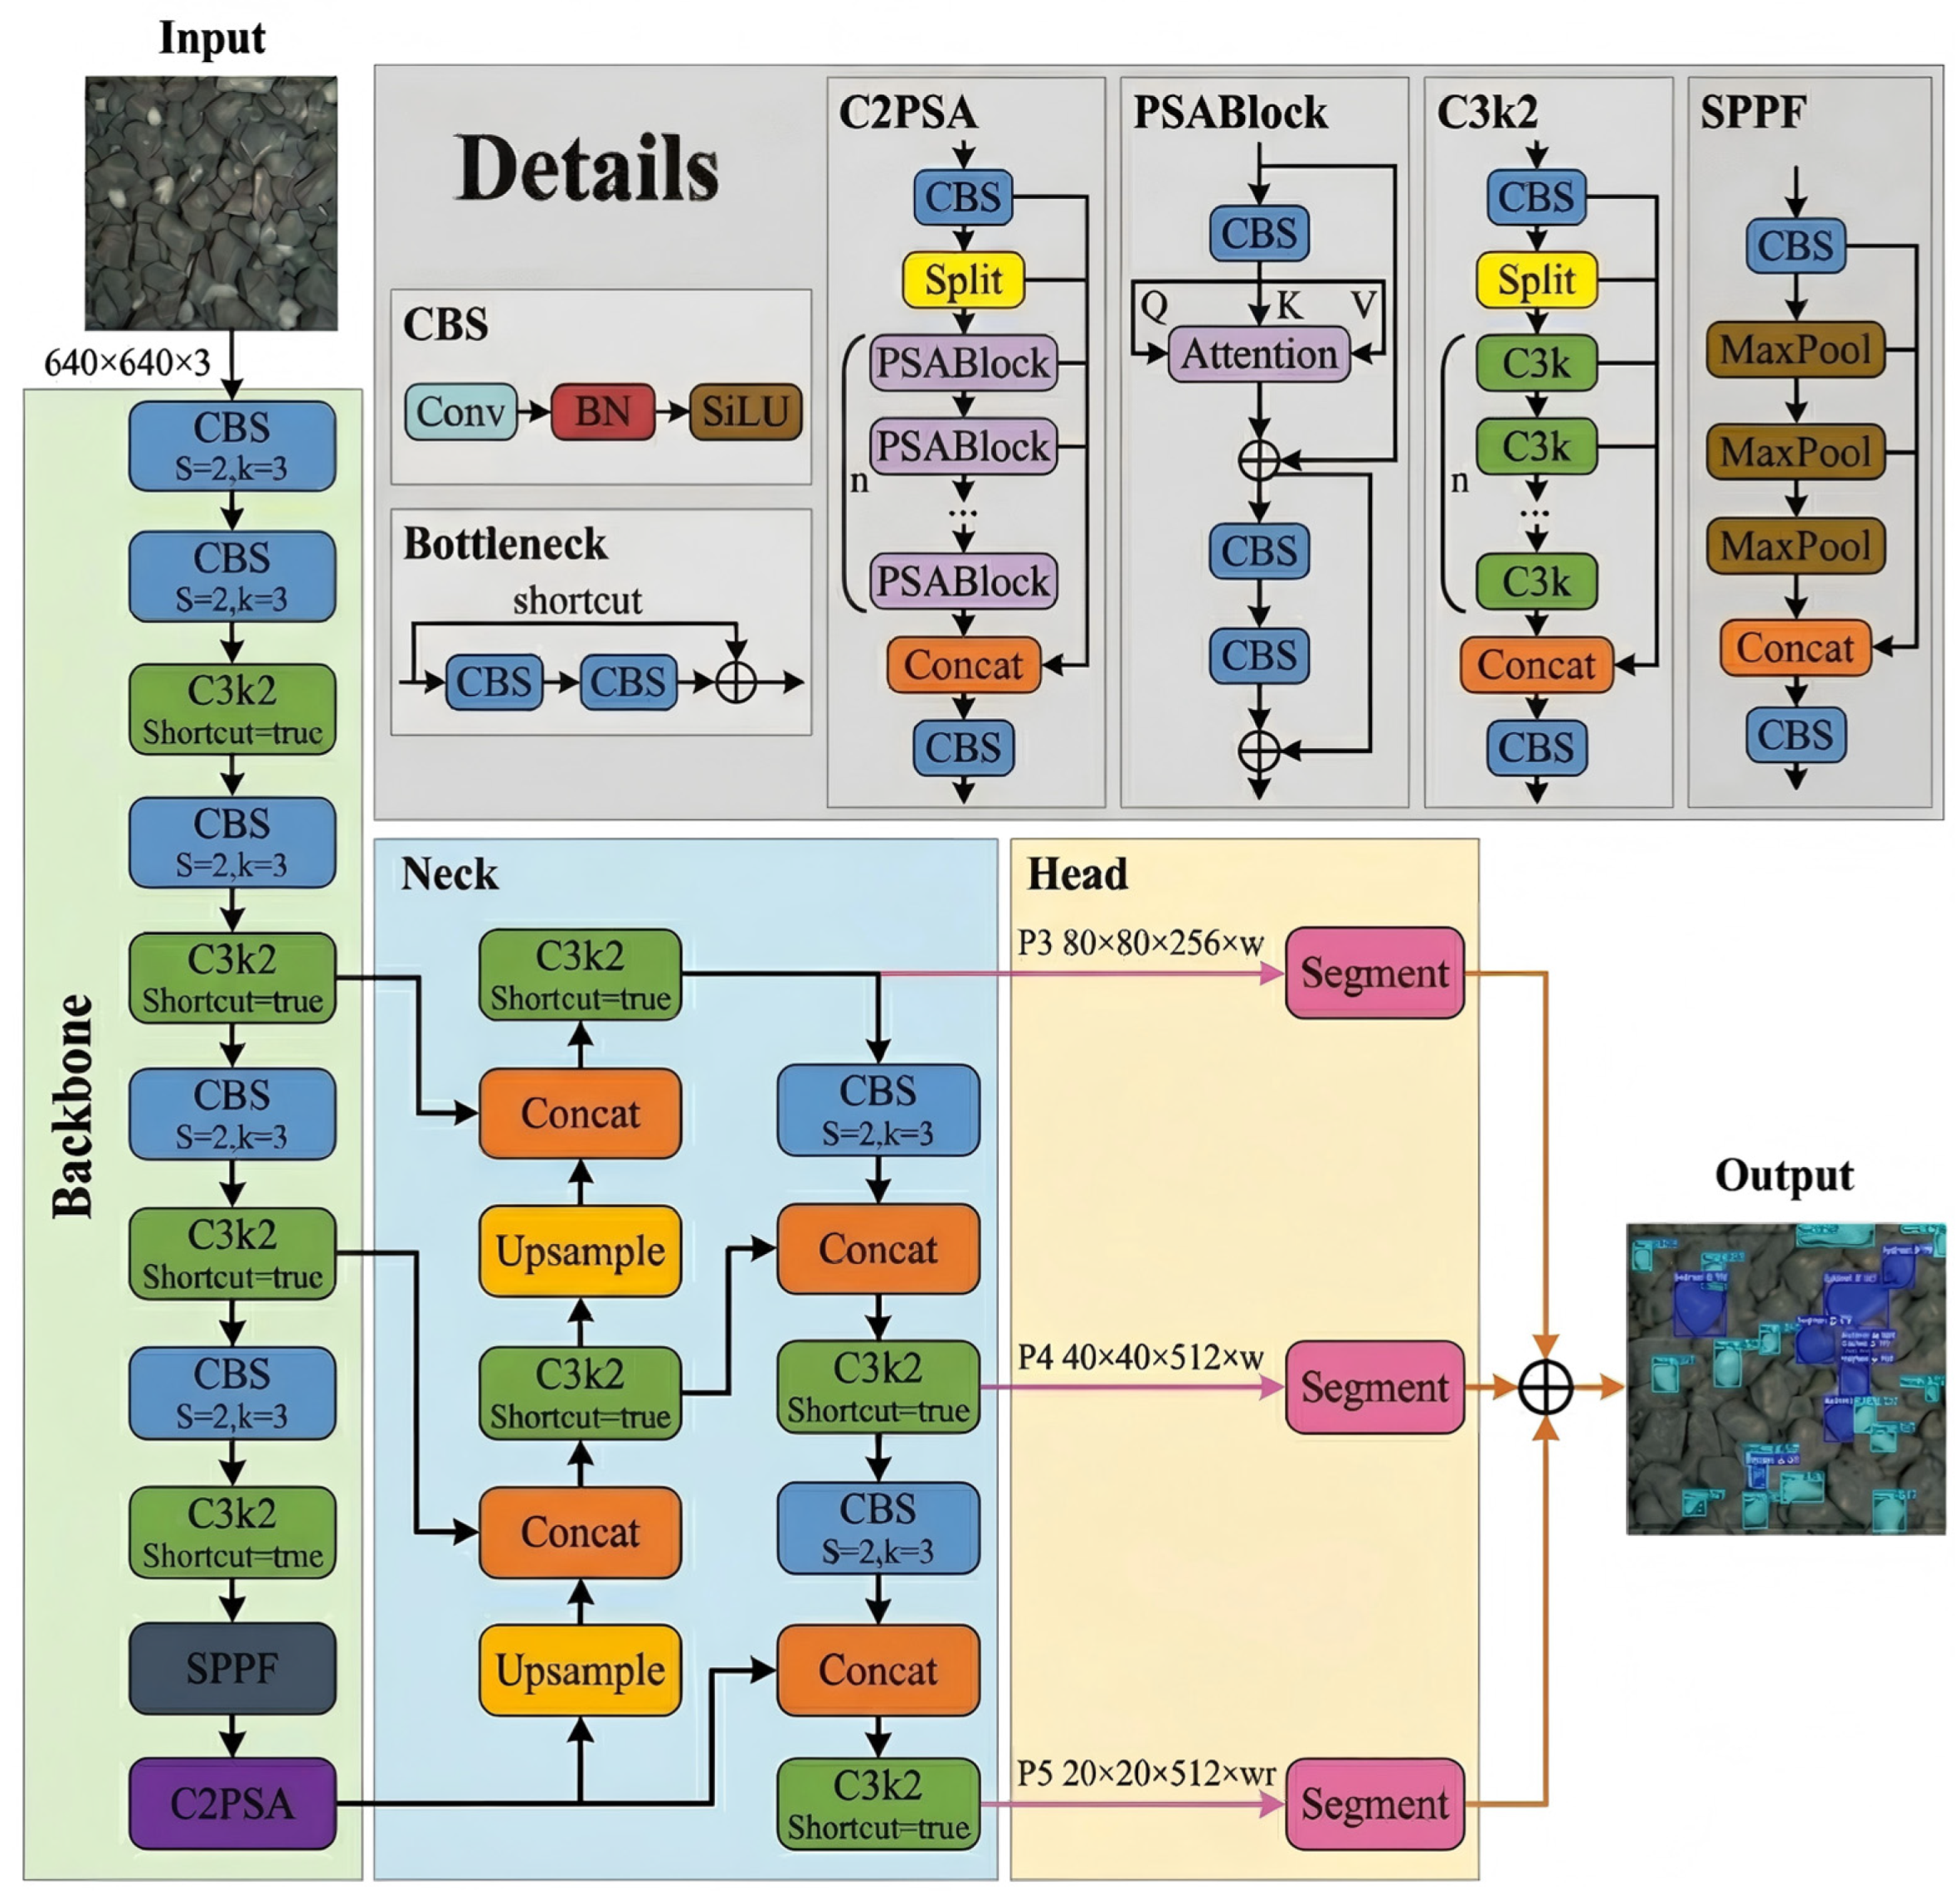
\includegraphics[width=\linewidth]{yolo11_seg_architecture.png}
\caption[Kiến trúc YOLO11-seg]{Kiến trúc YOLO11-seg, trích từ Hình~1 trong~\cite{wang2026lggyoloseg}. Kích thước ảnh đầu vào minh hoạ là $640 \times 640$.}
\label{fig:yolo11-arch}
\end{figure}

Trong hình, CBS gồm ba bước: Conv dùng bộ lọc để trích đặc trưng; BN điều chỉnh thang giá trị của các đặc trưng; SiLU biến đổi các giá trị qua hàm kích hoạt để mạng học được các quan hệ phức tạp. CBS tương ứng với khối Conv trong Bảng~\ref{tab:yolo_blocks}. Các ảnh đầu vào và đầu ra là ví dụ phân đoạn quặng của tài liệu nguồn. Bảng~\ref{tab:yolo_blocks} giải thích vai trò các khối chính của YOLO11-seg, theo tài liệu của Ultralytics~\cite{ultralytics_arch} và mã nguồn~\cite{yolo11}.

\begin{table}[H]
\centering
\caption{Vai trò của các khối trong YOLO11-seg}
\label{tab:yolo_blocks}
\begin{tabular}{>{\raggedright\arraybackslash}p{3.2cm} >{\raggedright\arraybackslash}p{11.8cm}}
\toprule
\textbf{Khối} & \textbf{Vai trò} \\
\midrule
Conv & Đơn vị cơ bản, lọc ảnh để lấy đặc trưng. Khi đặt bước nhảy 2, khối này giảm một nửa chiều cao và chiều rộng. \\
C3k2 & Khối lặp chính: cho một phần dữ liệu đi qua nhiều lớp xử lý, phần còn lại giữ nguyên rồi ghép lại, nhờ đó học được nhiều mà tốn ít phép tính. \\
SPPF & Gom thông tin từ các vùng rộng dần quanh mỗi vị trí, để mô hình nắm được ngữ cảnh xung quanh. \\
C2PSA & Dùng cơ chế chú ý (attention) để mỗi vị trí có thể tham khảo toàn ảnh và tập trung vào vùng có đối tượng. \\
Upsample, Concat & Phóng to bản đồ đặc trưng rồi ghép với bản đồ cùng kích thước. Neck dùng cách này theo hai chiều: đưa thông tin nhận dạng từ tầng sâu xuống và đưa thông tin vị trí từ tầng nông lên. \\
Segment & Tại mỗi vị trí trên ba mức đặc trưng, dự đoán hộp bao, điểm của từng lớp và 32 hệ số để dựng mặt nạ. \\
Proto & Sinh 32 \emph{mặt nạ nguyên mẫu}, là các mẫu trung gian dùng chung để tạo mặt nạ riêng cho từng đối tượng, không phải các lớp xe. \\
\bottomrule
\end{tabular}
\end{table}

Sau khi mô hình dự đoán, Non-Maximum Suppression (NMS) loại bỏ các dự đoán trùng nhau trên cùng một xe.
Mỗi xe còn lại có 32 hệ số riêng, cho biết mức đóng góp của từng mặt nạ nguyên mẫu. Mặt nạ của xe được tạo bằng cách cộng các nguyên mẫu theo những hệ số này, rồi cắt theo hộp bao, phóng về kích thước ảnh gốc và giữ các điểm ảnh có giá trị từ 0,5 trở lên.

Đồ án so sánh sơ bộ hai mô hình huấn luyện sẵn là YOLO11n-seg (nano) và YOLO11l-seg (large), rồi chọn một mô hình cho các thí nghiệm (mục~\ref{sec:model_select}). Hai mô hình có cùng sơ đồ khối ở Hình~\ref{fig:yolo11-arch}, chỉ khác về độ lớn~\cite{yolo11}.
Bản large có số tham số gấp gần 10 lần bản nano, nên nhận dạng tốt hơn nhưng chạy chậm hơn.

COCO (Common Objects in Context)~\cite{lin2014coco} là bộ dữ liệu ảnh công khai gồm 80 lớp đối tượng thường gặp, được dùng rộng rãi để huấn luyện và so sánh các mô hình. Bộ này chứa sẵn các lớp \texttt{car}, \texttt{truck}, \texttt{bus}, \texttt{motorcycle}, nên đồ án có thể dùng mô hình huấn luyện sẵn và chỉ giữ bốn lớp này khi inference (chạy mô hình để dự đoán).

Thư viện Ultralytics cung cấp tập điểm biên của từng mặt nạ qua thuộc tính \texttt{masks.xy}; đồ án sử dụng tập điểm này làm đầu vào cho thuật toán dựng bao lồi trực giao.

% =====================================================================
\section{Bao lồi trực giao}
\label{sec:och}

\subsection{Các khái niệm}

\begin{dinhnghia}[Tập lồi]
Tập $K$ trong mặt phẳng được gọi là \emph{lồi} nếu với hai điểm bất kỳ thuộc $K$, toàn bộ đoạn thẳng nối chúng cũng thuộc $K$.
\end{dinhnghia}
Nói đơn giản, khi nối hai điểm trong tập bằng một đoạn thẳng, đoạn nối không đi ra ngoài tập.

\begin{dinhnghia}[Bao lồi]
\emph{Bao lồi} của tập điểm $P$, ký hiệu $\operatorname{conv}(P)$, là tập lồi nhỏ nhất chứa $P$.
\end{dinhnghia}
Có thể hình dung căng một sợi dây thun quanh các điểm rồi thả ra: dây ôm sát các điểm ngoài cùng, còn dây và phần bên trong tạo thành bao lồi.

Trước khi định nghĩa bao lồi trực giao, một tập được gọi là \emph{lồi trực giao} nếu giao của nó với mỗi đường thẳng ngang hoặc dọc là tập rỗng, một điểm, hoặc một đoạn thẳng. Nói đơn giản, mỗi đường ngang hoặc dọc chỉ cắt tập thành nhiều nhất một đoạn liền, không thành hai đoạn rời nhau.

\begin{dinhnghia}[Bao lồi trực giao liên thông~\cite{an2021ograham,nguyen2022quickhull}]
Một bao lồi trực giao liên thông của tập điểm $P$ là một tập chứa tất cả các điểm của $P$, liền một khối, thoả mãn điều kiện lồi trực giao và không thể bỏ bớt phần nào mà vẫn giữ các tính chất này.
\end{dinhnghia}
Trong báo cáo, ``bao lồi trực giao liên thông'' được gọi tắt là ``bao lồi trực giao''.

\subsection{Cấu trúc bậc thang và đặc trưng hình học}
\label{sec:staircase}

Để hình dung cách dựng bao, trước hết xét các điểm nằm ở phía ngoài của tập điểm $P$. Từ một điểm $p$, kẻ một đường ngang và một đường dọc để chia mặt phẳng thành bốn góc phần tư: trên phải, trên trái, dưới trái và dưới phải, có tính cả các điểm nằm trên đường ngang hoặc dọc giới hạn góc đó. Nếu có ít nhất một góc phần tư không chứa điểm nào khác của $P$, thì $p$ được gọi là \emph{điểm tối đại}~\cite{nguyen2022quickhull}. Chẳng hạn, một điểm có góc phần tư trên trái trống là điểm tối đại theo hướng Tây Bắc.

Từ tập điểm $P$, tìm vị trí trái nhất, phải nhất, thấp nhất và cao nhất. Kẻ hai đường dọc và hai đường ngang qua các vị trí này, ta được \emph{hình chữ nhật bao}. Đây là khung phụ để xác định các điểm mốc, chưa phải bao lồi trực giao.

Trên cạnh trên và cạnh dưới, lấy điểm trái nhất và phải nhất; trên cạnh trái và cạnh phải, lấy điểm cao nhất và thấp nhất. Như vậy có tối đa tám \emph{điểm mốc}. Nếu một cạnh chỉ có một điểm thì hai mốc trên cạnh đó trùng nhau; điểm nằm ở góc hình chữ nhật cũng có thể là mốc của hai cạnh.

Biên của bao được chia thành bốn phần ở bốn góc, mỗi phần có dạng bậc thang (Hình~\ref{fig:four_chains}):
\begin{itemize}
  \item \textbf{Góc trên trái (Tây Bắc):} nối điểm trái nhất trên cạnh trên với điểm cao nhất trên cạnh trái.
  \item \textbf{Góc dưới trái (Tây Nam):} nối điểm thấp nhất trên cạnh trái với điểm trái nhất trên cạnh dưới.
  \item \textbf{Góc dưới phải (Đông Nam):} nối điểm phải nhất trên cạnh dưới với điểm thấp nhất trên cạnh phải.
  \item \textbf{Góc trên phải (Đông Bắc):} nối điểm cao nhất trên cạnh phải với điểm phải nhất trên cạnh trên.
\end{itemize}
Mỗi phần được gọi là một \emph{chuỗi bậc thang}. Bốn chuỗi, ghép với các đoạn nối trên bốn cạnh hình chữ nhật, tạo thành đường viền của bao.

\begin{figure}[H]
\centering
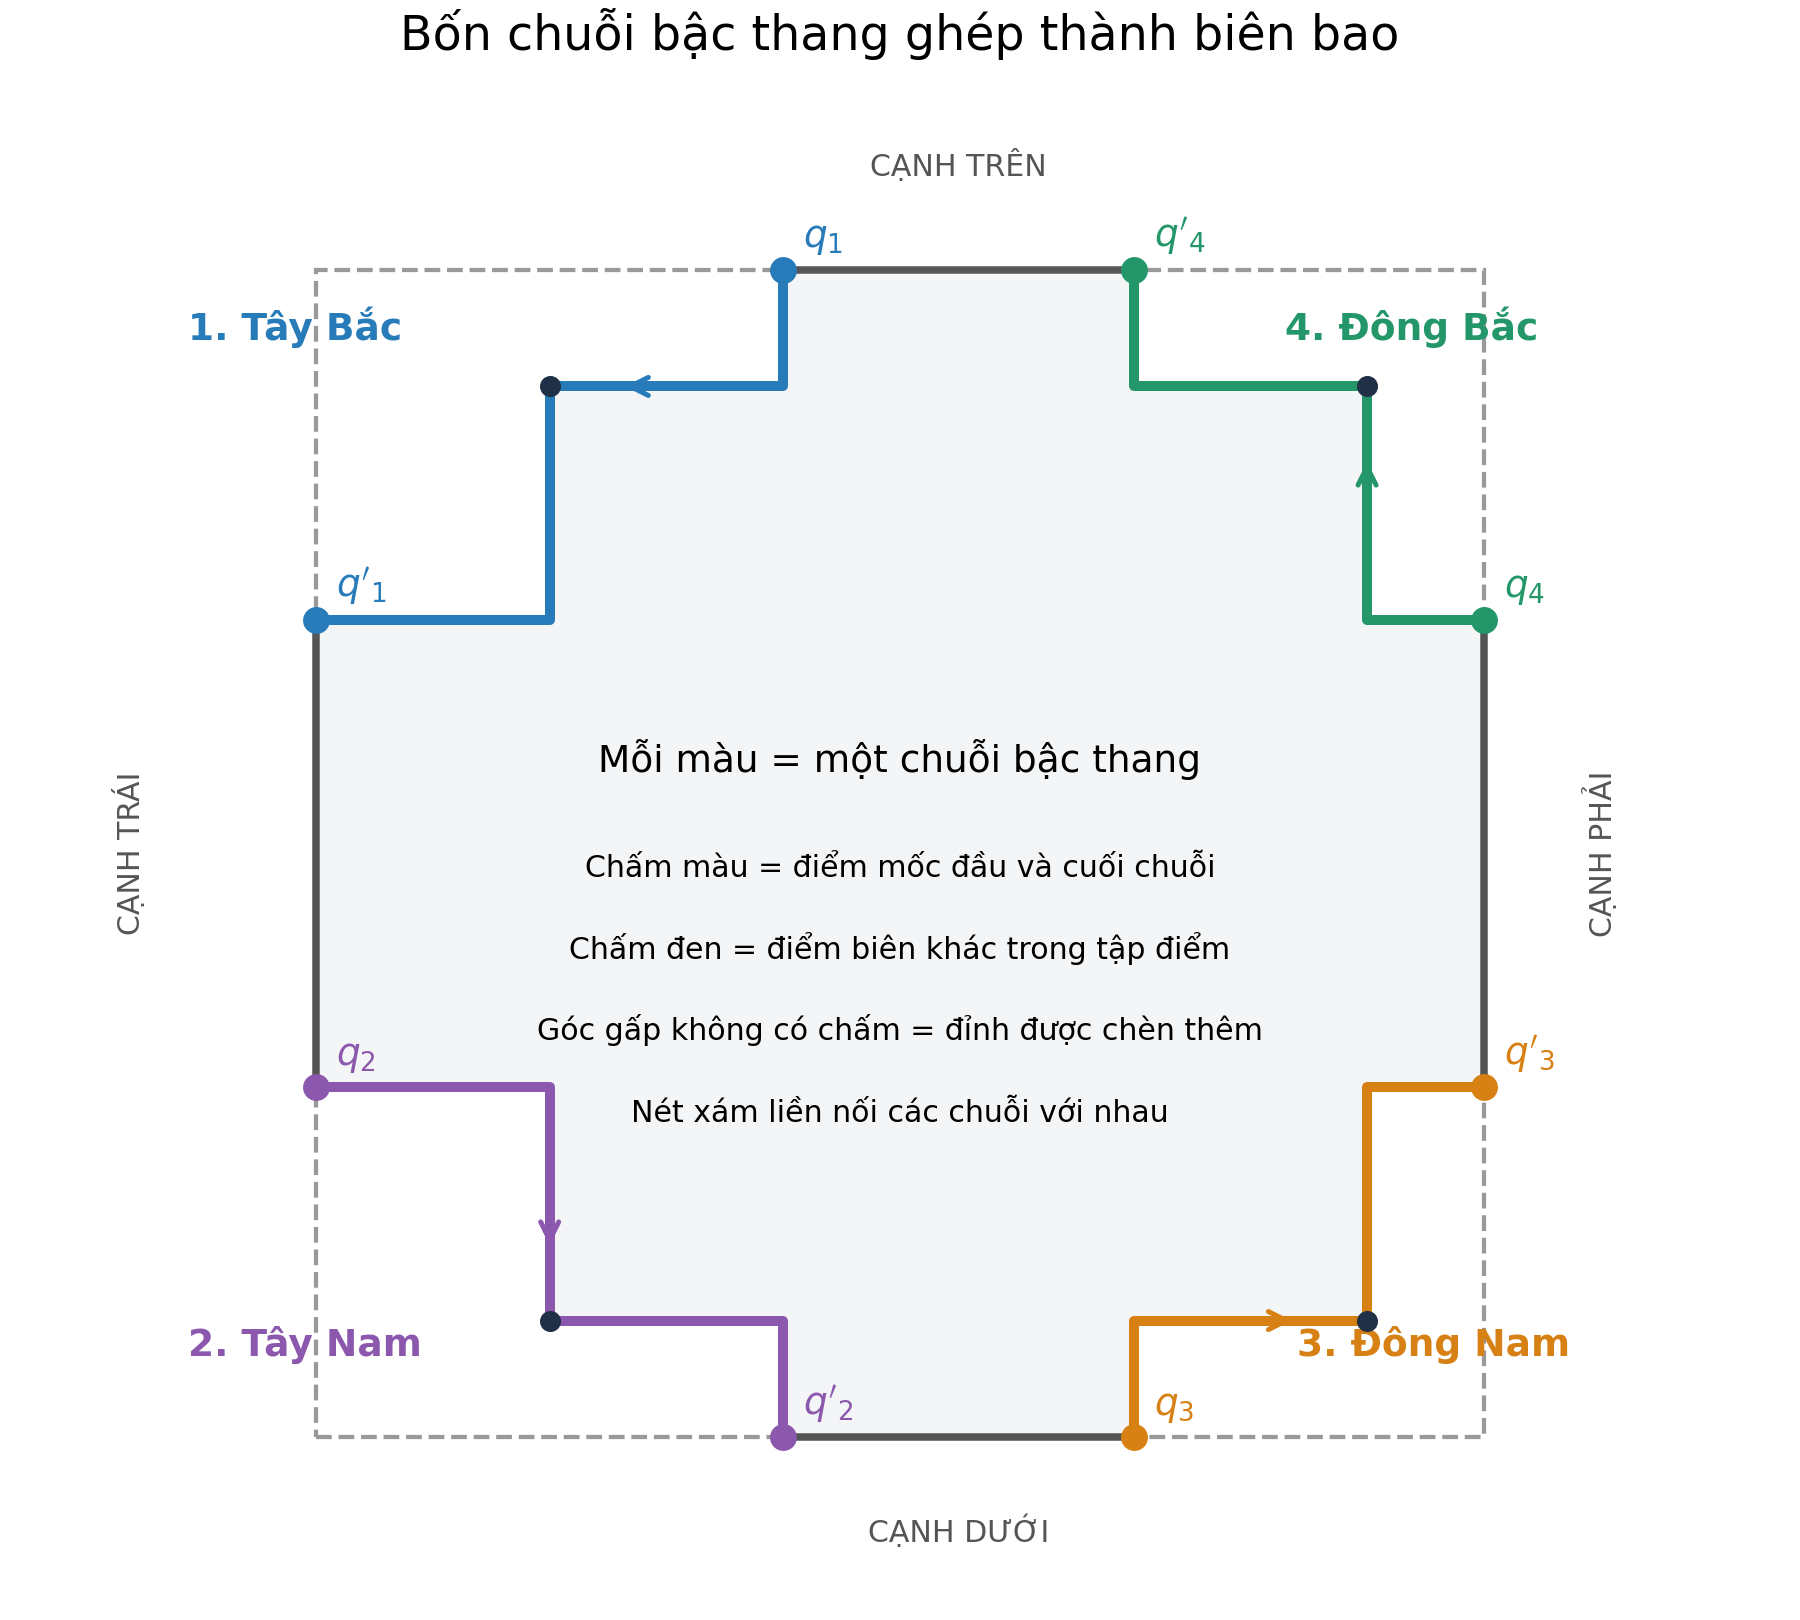
\includegraphics[width=0.92\linewidth]{four_staircase_chains.png}
\caption{Minh hoạ bốn chuỗi bậc thang bằng bốn màu. Các chấm màu là điểm mốc đầu và cuối chuỗi; các đoạn xám liền nối các chuỗi. Khung nét đứt là hình chữ nhật bao.}
\label{fig:four_chains}
\end{figure}

Các điểm của $P$ được chọn trên mỗi chuỗi là điểm tối đại theo hướng tương ứng~\cite{nguyen2022quickhull}. Khi hai điểm liên tiếp nằm chéo nhau, ta nối chúng bằng một đoạn ngang và một đoạn dọc. Chỗ rẽ là một góc vuông được chèn thêm về phía trong bao, không nhất thiết thuộc $P$. Trong Hình~\ref{fig:four_chains}, các góc gấp không có chấm chính là những đỉnh được chèn thêm. Hình~\ref{fig:hull_illus} minh hoạ kết quả trên một tập 28 điểm.

\begin{figure}[H]
\centering
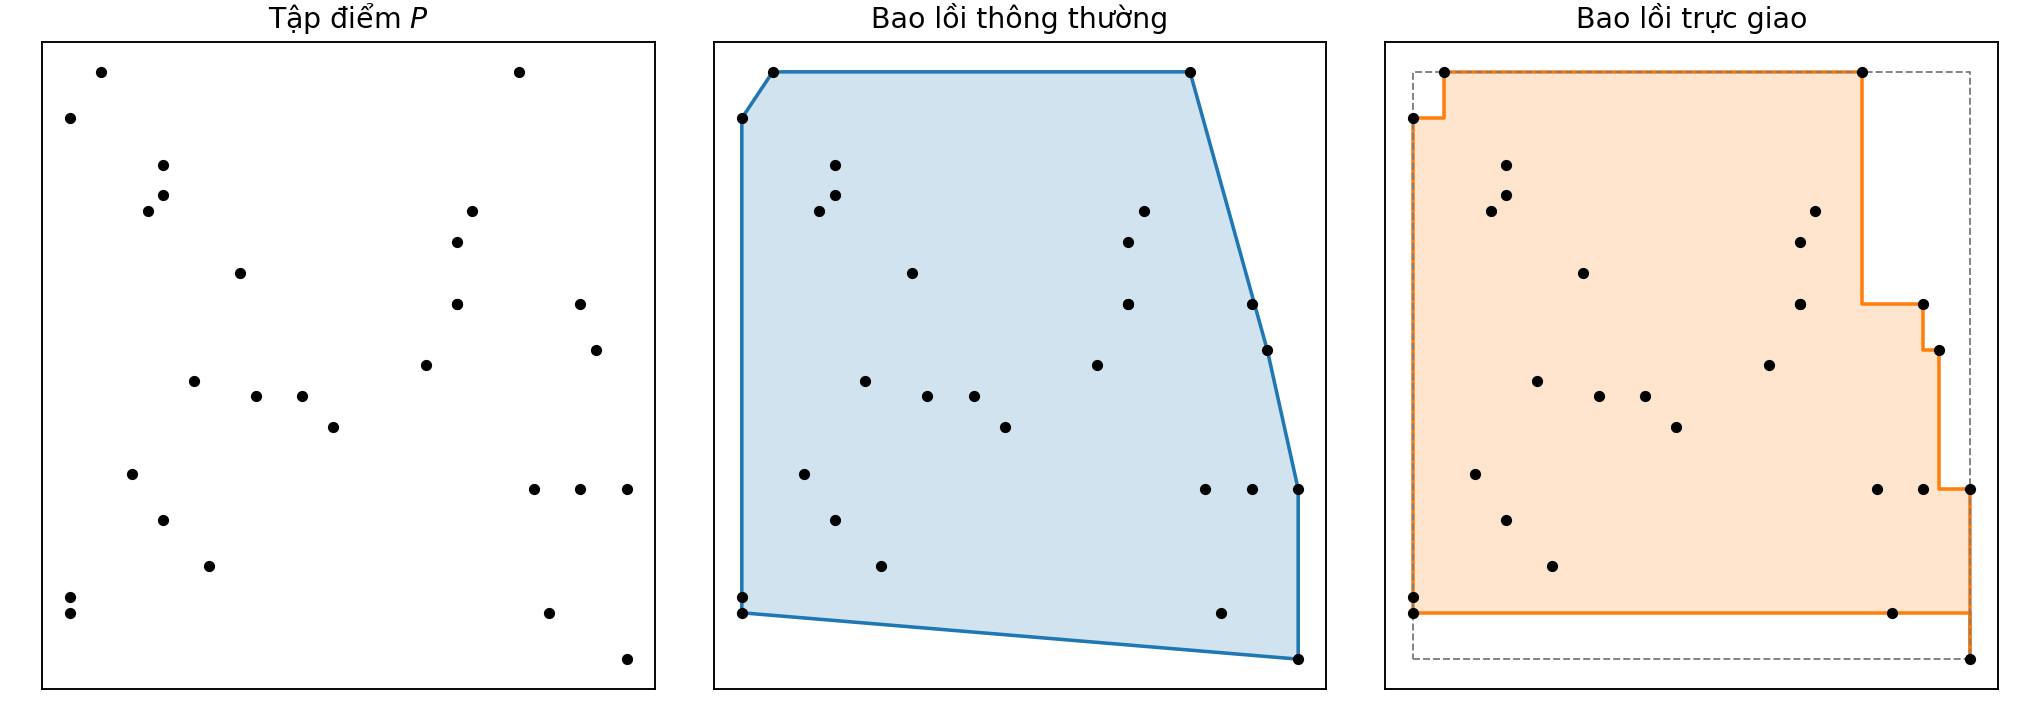
\includegraphics[width=0.98\linewidth]{hull_illustration.png}
\caption{Một tập điểm (trái), bao lồi thông thường (giữa) và bao lồi trực giao liên thông (phải); nét đứt là hình
chữ nhật bao. Đoạn thẳng đứng ở góc dưới phải nối điểm thấp nhất vào phần còn lại của bao; đa giác trực giao trong~\cite{nguyen2022quickhull} cho phép có các đoạn thẳng như vậy.}
\label{fig:hull_illus}
\end{figure}

\begin{nhanxet}
\label{rem:inclusion}
Bao lồi trực giao liên thông và bao lồi thông thường đều chứa $P$ và đều nằm trong hình chữ nhật bao.
Tuy nhiên, bao trực giao liên thông không phải lúc nào cũng nằm trong bao lồi thông thường:
khi các điểm thẳng hàng theo đường chéo, bao lồi chỉ là một đoạn thẳng, còn đường nối trực giao phải đi ra ngoài đoạn đó.
Vì vậy, mức nền thừa và khả năng biểu diễn hình dạng của các loại bao
cần được so sánh bằng thực nghiệm trên dữ liệu cụ thể; kết quả của đồ án được trình bày ở Chương~\ref{chap:exp}.
\end{nhanxet}

Diện tích của đa giác bao được tính từ toạ độ các đỉnh, còn chu vi là tổng độ dài các cạnh.
Trong đầu ra video, tỉ lệ lấp đầy được tính bằng diện tích bao chia cho diện tích hộp phát hiện YOLO, cho biết vùng bao chiếm bao nhiêu phần của hộp. Hộp YOLO được mô hình dự đoán riêng, nên có thể khác hình chữ nhật tính từ các điểm biên. Các đối tượng có dựng bao được lưu những đặc trưng này vào tệp CSV (bảng dữ liệu dạng văn bản).

% =====================================================================
\paragraph{Tính duy nhất của bao.}
Một tập điểm có thể có nhiều bao lồi trực giao liên thông hợp lệ~\cite{an2021ograham,nguyen2022quickhull}. Hai bản cài đặt dùng quy tắc nối cố định để tạo đầu ra. Quy tắc nối cố định không tự bảo đảm bao tối tiểu và duy nhất trên mọi tập điểm.

\section{Bản QuickHull của nhóm}
\label{sec:quickhull}

QuickHull là ý tưởng tìm biên bằng cách chọn điểm rồi tiếp tục xử lý các tập điểm nhỏ hơn~\cite{eddy1977,barber1996}. O-Quickhull áp dụng ý tưởng chia để trị cho bao lồi trực giao~\cite{nguyen2022quickhull}. Đồ án dùng một bản QuickHull chọn điểm theo toạ độ, không tái hiện bước chọn điểm xa góc gấp nhất và chia hai nhánh của O-Quickhull gốc. Các bước, giả mã và hình trong mục này mô tả bản cài đặt thực tế của nhóm. Trong báo cáo, hai bản cài đặt được gọi ngắn là \emph{bản QuickHull} (bản đệ quy chọn điểm theo toạ độ) và \emph{bản Graham} (bản sắp xếp--quét theo ý tưởng O-Graham); các tên ngắn này không khẳng định nhóm tái hiện nguyên thuật toán gốc.

Trong bản QuickHull này, việc chọn điểm theo toạ độ có nghĩa là chọn điểm có toạ độ cao nhất, thấp nhất, trái nhất hoặc phải nhất theo hướng đang xét. Đây là cách chọn theo toạ độ, không phải khẳng định mọi điểm được chọn đều là điểm cực trị của bao trên mọi đầu vào.

Trước hết, tìm tối đa tám điểm mốc và chia tập điểm thành bốn vùng ứng với bốn chuỗi bậc thang ở mục~\ref{sec:staircase}. Gọi hai mốc đầu--cuối của chuỗi thứ $k$ là $(q_k,q'_k)$, với $k=1,2,3,4$ lần lượt ứng với Tây Bắc, Tây Nam, Đông Nam và Đông Bắc.

Với chuỗi Tây Bắc, bản cài đặt xử lý như sau:
\begin{enumerate}
  \item \textbf{Lấy tập điểm cần xét.} Giữ các điểm trong hình chữ nhật có hai đỉnh đối diện là hai mốc của chuỗi, bỏ chính hai mốc. Gọi tập này là $S$; nếu $S$ rỗng thì không cần tìm thêm điểm trung gian.
  \item \textbf{Chọn hai điểm theo toạ độ.} Chọn điểm cao nhất của $S$; nếu có nhiều điểm cùng độ cao thì lấy điểm bên trái nhất. Tiếp đó, chọn điểm trái nhất của $S$; nếu có nhiều điểm cùng vị trí ngang thì lấy điểm cao nhất. Mã thực hiện việc này bằng hai lần sắp xếp.
  \item \textbf{Thu hẹp tập cần xử lý.} Giữ các điểm trong hình chữ nhật giữa hai điểm vừa chọn, bỏ chính hai điểm đó. Áp dụng lại bước chọn điểm cho tập nhỏ hơn này. Mỗi lần chỉ có một lời gọi tiếp theo; đó là đệ quy một nhánh.
  \item \textbf{Ghép kết quả.} Xếp điểm cao nhất trước, kết quả của lời gọi tiếp theo ở giữa và điểm trái nhất sau. Đưa hai mốc ban đầu vào đầu--cuối chuỗi, rồi chèn góc ngang--dọc giữa các điểm nằm chéo nhau. Các điểm liên tiếp bị trùng được loại ở bước chuẩn hoá chung.
\end{enumerate}

Hình~\ref{fig:recursive_steps} minh hoạ trên một tập điểm cụ thể. Hai điểm được chọn trong cùng một lời gọi có thể trùng nhau: ở bước cuối của ví dụ, điểm $c$ vừa cao nhất vừa trái nhất trong tập đang xét.

\begin{figure}[H]
\centering
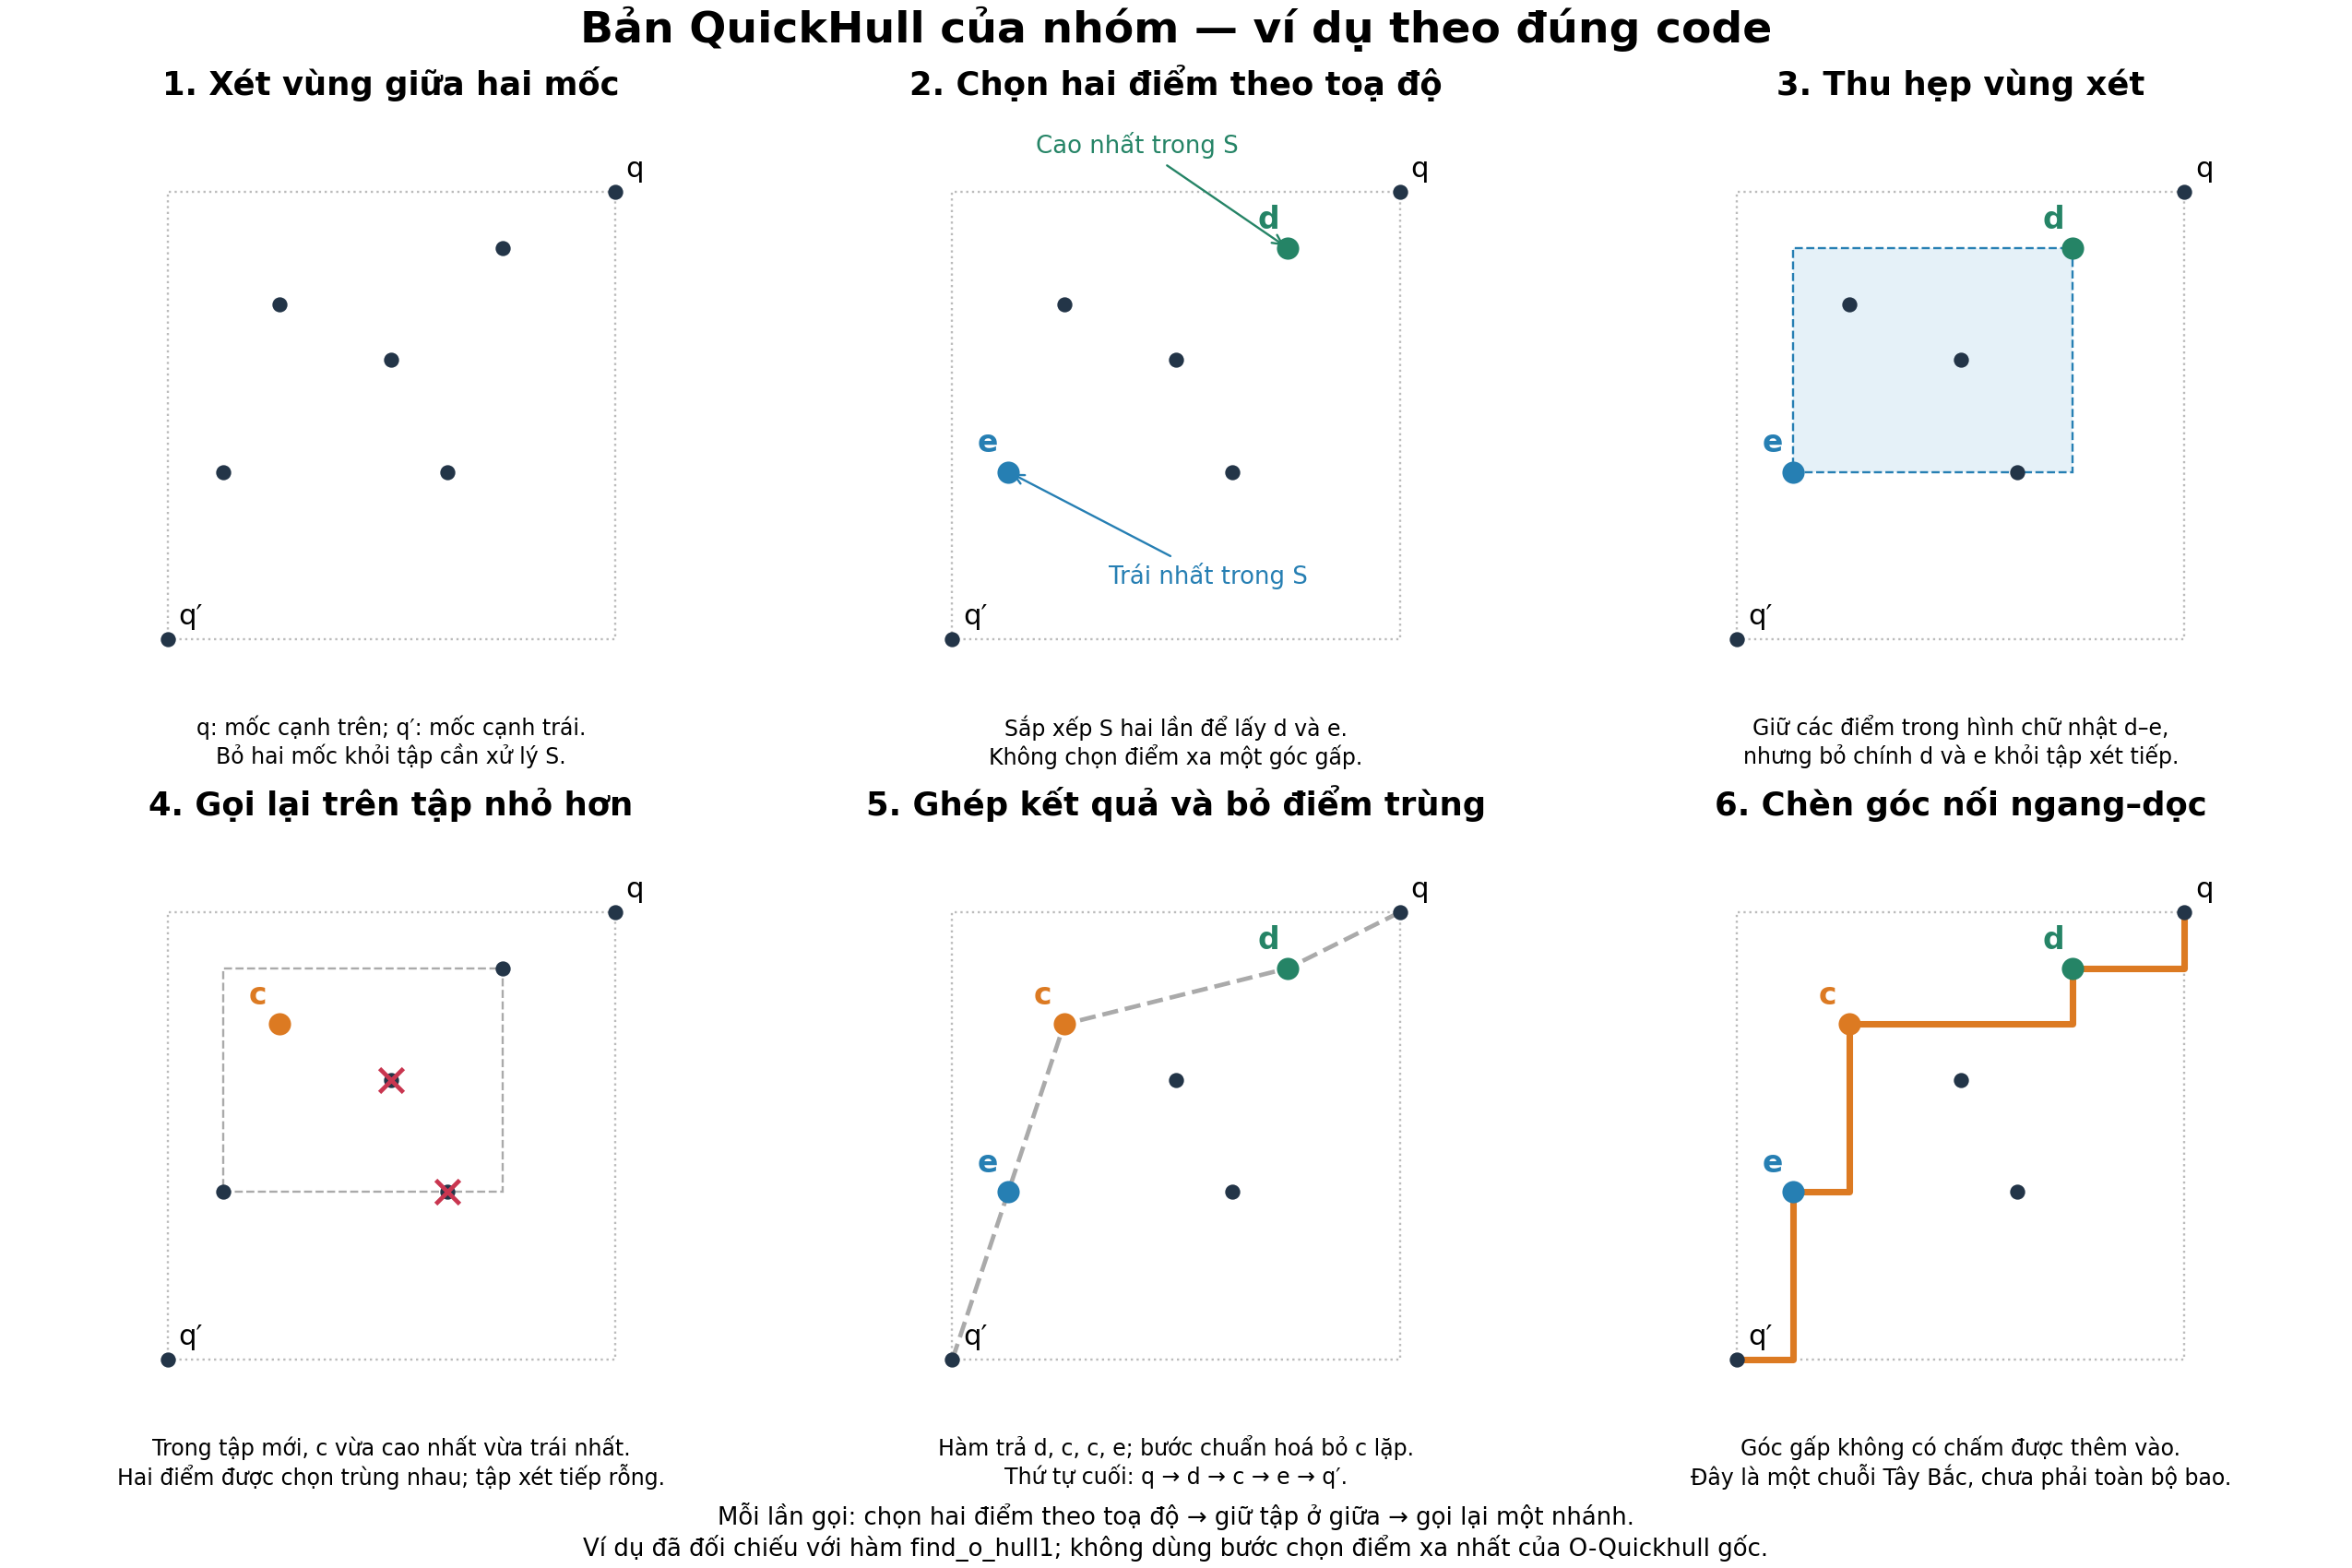
\includegraphics[width=\linewidth]{recursive_group_steps.png}
\caption[Minh hoạ bản QuickHull của nhóm]{Các bước tìm chuỗi Tây Bắc theo bản cài đặt của nhóm. Mã chọn $d$ cao nhất và $e$ trái nhất, rồi xử lý tập nằm giữa chúng để tìm $c$. Sau khi bỏ điểm trùng, các điểm được ghép theo thứ tự $q,d,c,e,q'$ và chèn góc nối. Hình chỉ minh hoạ một chuỗi, chưa phải toàn bộ bao.}
\label{fig:recursive_steps}
\end{figure}

Trong giả mã QuickHull, $A$ là dãy kết quả ghép bốn chuỗi; $S_k$ là tập điểm nằm giữa hai mốc của chuỗi thứ $k$, không gồm hai mốc. Ký hiệu $[]$ là dãy rỗng. Hàm tìm chuỗi của bản QuickHull chỉ trả về các điểm trung gian; phần chính đưa hai mốc vào đầu và cuối. Chỉ số $k=1,2,3,4$ lần lượt ứng với Tây Bắc, Tây Nam, Đông Nam và Đông Bắc. Ký hiệu $\operatorname{Rect}(a,b)$ là hình chữ nhật có hai đỉnh đối diện $a,b$. Ký hiệu $\operatorname{Inside}(S,a,b)$ chỉ các điểm của $S$ nằm trong hoặc trên biên hình chữ nhật này, nhưng không gồm chính $a,b$:
\[
\operatorname{Inside}(S,a,b)=\{p\in S\setminus\{a,b\}:p\in\operatorname{Rect}(a,b)\}.
\]

\begin{algorithm}[H]
\SetAlgoLined
\LinesNumbered
\caption{Bản QuickHull (cài đặt của nhóm)}
\label{alg:quickhull}
\KwIn{Tập điểm $P$, $|P|=n\ge 4$}
\KwOut{Dãy đỉnh của bao lồi trực giao liên thông, theo thứ tự quanh biên}
Tìm $x_{\min},x_{\max},y_{\min},y_{\max}$ và các mốc $q_1,q'_1,\dots,q_4,q'_4$\;
\For{$k\gets 1$ \KwTo $4$}{
  $S_k\gets\operatorname{Inside}(P,q_k,q'_k)$ \tcp*{các điểm giữa hai mốc, không gồm hai mốc}
}
$A\gets []$\;
\For{$k\gets 1$ \KwTo $4$}{
  Nối vào $A$: $q_k$, $\textsc{FindChain}_k(S_k)$, $q'_k$\;
}
Với mỗi cặp đỉnh liên tiếp của $A$ khác nhau ở cả hai toạ độ, chèn một đỉnh góc $90^\circ$\;
\Return $A$\;
\BlankLine
\SetKwFunction{FC}{FindChain$_1$}
\SetKwProg{Fn}{Hàm}{:}{}
\Fn{\FC{$S$}}{
  \If{$S=\emptyset$}{\Return dãy rỗng}
  $a\gets$ điểm cao nhất của $S$ (nếu bằng nhau, lấy điểm bên trái nhất) \tcp*{sắp xếp $S$}
  $b\gets$ điểm trái nhất của $S$ (nếu bằng nhau, lấy điểm cao nhất) \tcp*{sắp xếp $S$}
  \Return $a$, \FC{$\operatorname{Inside}(S,a,b)$}, $b$\;
}
\end{algorithm}

Ba hàm $\textsc{FindChain}_2$, $\textsc{FindChain}_3$, $\textsc{FindChain}_4$ có cùng cách thu hẹp tập điểm, nhưng đổi hướng chọn điểm cho các chuỗi Tây Nam, Đông Nam và Đông Bắc. Độ phức tạp của hai bản cài đặt được tóm tắt trong Bảng~\ref{tab:algo_compare}.

% =====================================================================
\section{Bản Graham của nhóm}
\label{sec:ograham}
\label{sec:impl_ograham}

Thuật toán Graham~\cite{graham1972} tìm bao lồi bằng cách sắp xếp các điểm rồi quét một lượt duy nhất.
Phan Thanh An và cộng sự~\cite{an2021ograham} cải biên ý tưởng này cho bao lồi trực giao liên thông (gọi tắt là \emph{O-Graham}):
thay vì sắp xếp theo góc, các điểm được sắp xếp theo toạ độ; thay vì kiểm tra rẽ trái/rẽ phải,
chỉ cần so sánh một toạ độ để biết điểm có nằm trên chuỗi bậc thang hay không.

Để minh hoạ cách sắp xếp và quét, Thuật toán~\ref{alg:ograham} trình bày bản cài đặt của nhóm theo ý tưởng O-Graham. Đây không phải giả mã sao chép từ bài báo gốc; nhóm chưa đối chiếu từng bước để khẳng định hai bản hoàn toàn tương đương. Trong giả mã, $(s,e)$ là hai mốc đầu--cuối của chuỗi đang xét; $R$ là tập điểm trong hình chữ nhật giữa hai mốc; $C$ là dãy điểm được giữ cho chuỗi đó; $H$ là dãy kết quả ghép bốn chuỗi. Ký hiệu $\operatorname{last}(C)$ là điểm cuối của $C$. Khoá sắp xếp là thứ tự ưu tiên các toạ độ khi xếp điểm, được nêu cho cả bốn hướng ở Bảng~\ref{tab:scan_keys}.

Với chuỗi Tây Bắc, bản Graham của nhóm thực hiện theo các bước sau:
\begin{enumerate}
  \item \textbf{Lấy vùng cần xét.} Giữ các điểm nằm trong hình chữ nhật giữa hai mốc của chuỗi; bắt đầu dãy kết quả bằng mốc trên cạnh trên.
  \item \textbf{Sắp xếp vùng một lần.} Xếp điểm từ cao xuống thấp; các điểm cùng độ cao được xếp từ trái sang phải.
  \item \textbf{Duyệt theo thứ tự đã sắp.} Chỉ thêm một điểm nếu nó nằm bên trái điểm cuối đang giữ. Vì các điểm cùng độ cao đã được xếp từ trái sang phải, chỉ điểm trái nhất của hàng đó có thể được thêm; các điểm còn lại tự không thoả điều kiện đi xa hơn về trái. Nhờ đó, chuỗi tiến dần từ cạnh trên sang cạnh trái.
  \item \textbf{Hoàn thiện chuỗi.} Sau khi duyệt hết vùng, chèn các góc ngang--dọc giữa những điểm nằm chéo nhau. Làm tương tự cho ba hướng còn lại với thứ tự sắp xếp và hướng so sánh tương ứng.
\end{enumerate}

Hình~\ref{fig:ograham_steps} dùng cùng tập điểm với Hình~\ref{fig:recursive_steps}. Hai cách cho cùng chuỗi trong ví dụ, nhưng bản Graham không gọi đệ quy và không sắp xếp lại tập điểm ở từng bước duyệt.

\begin{figure}[H]
\centering
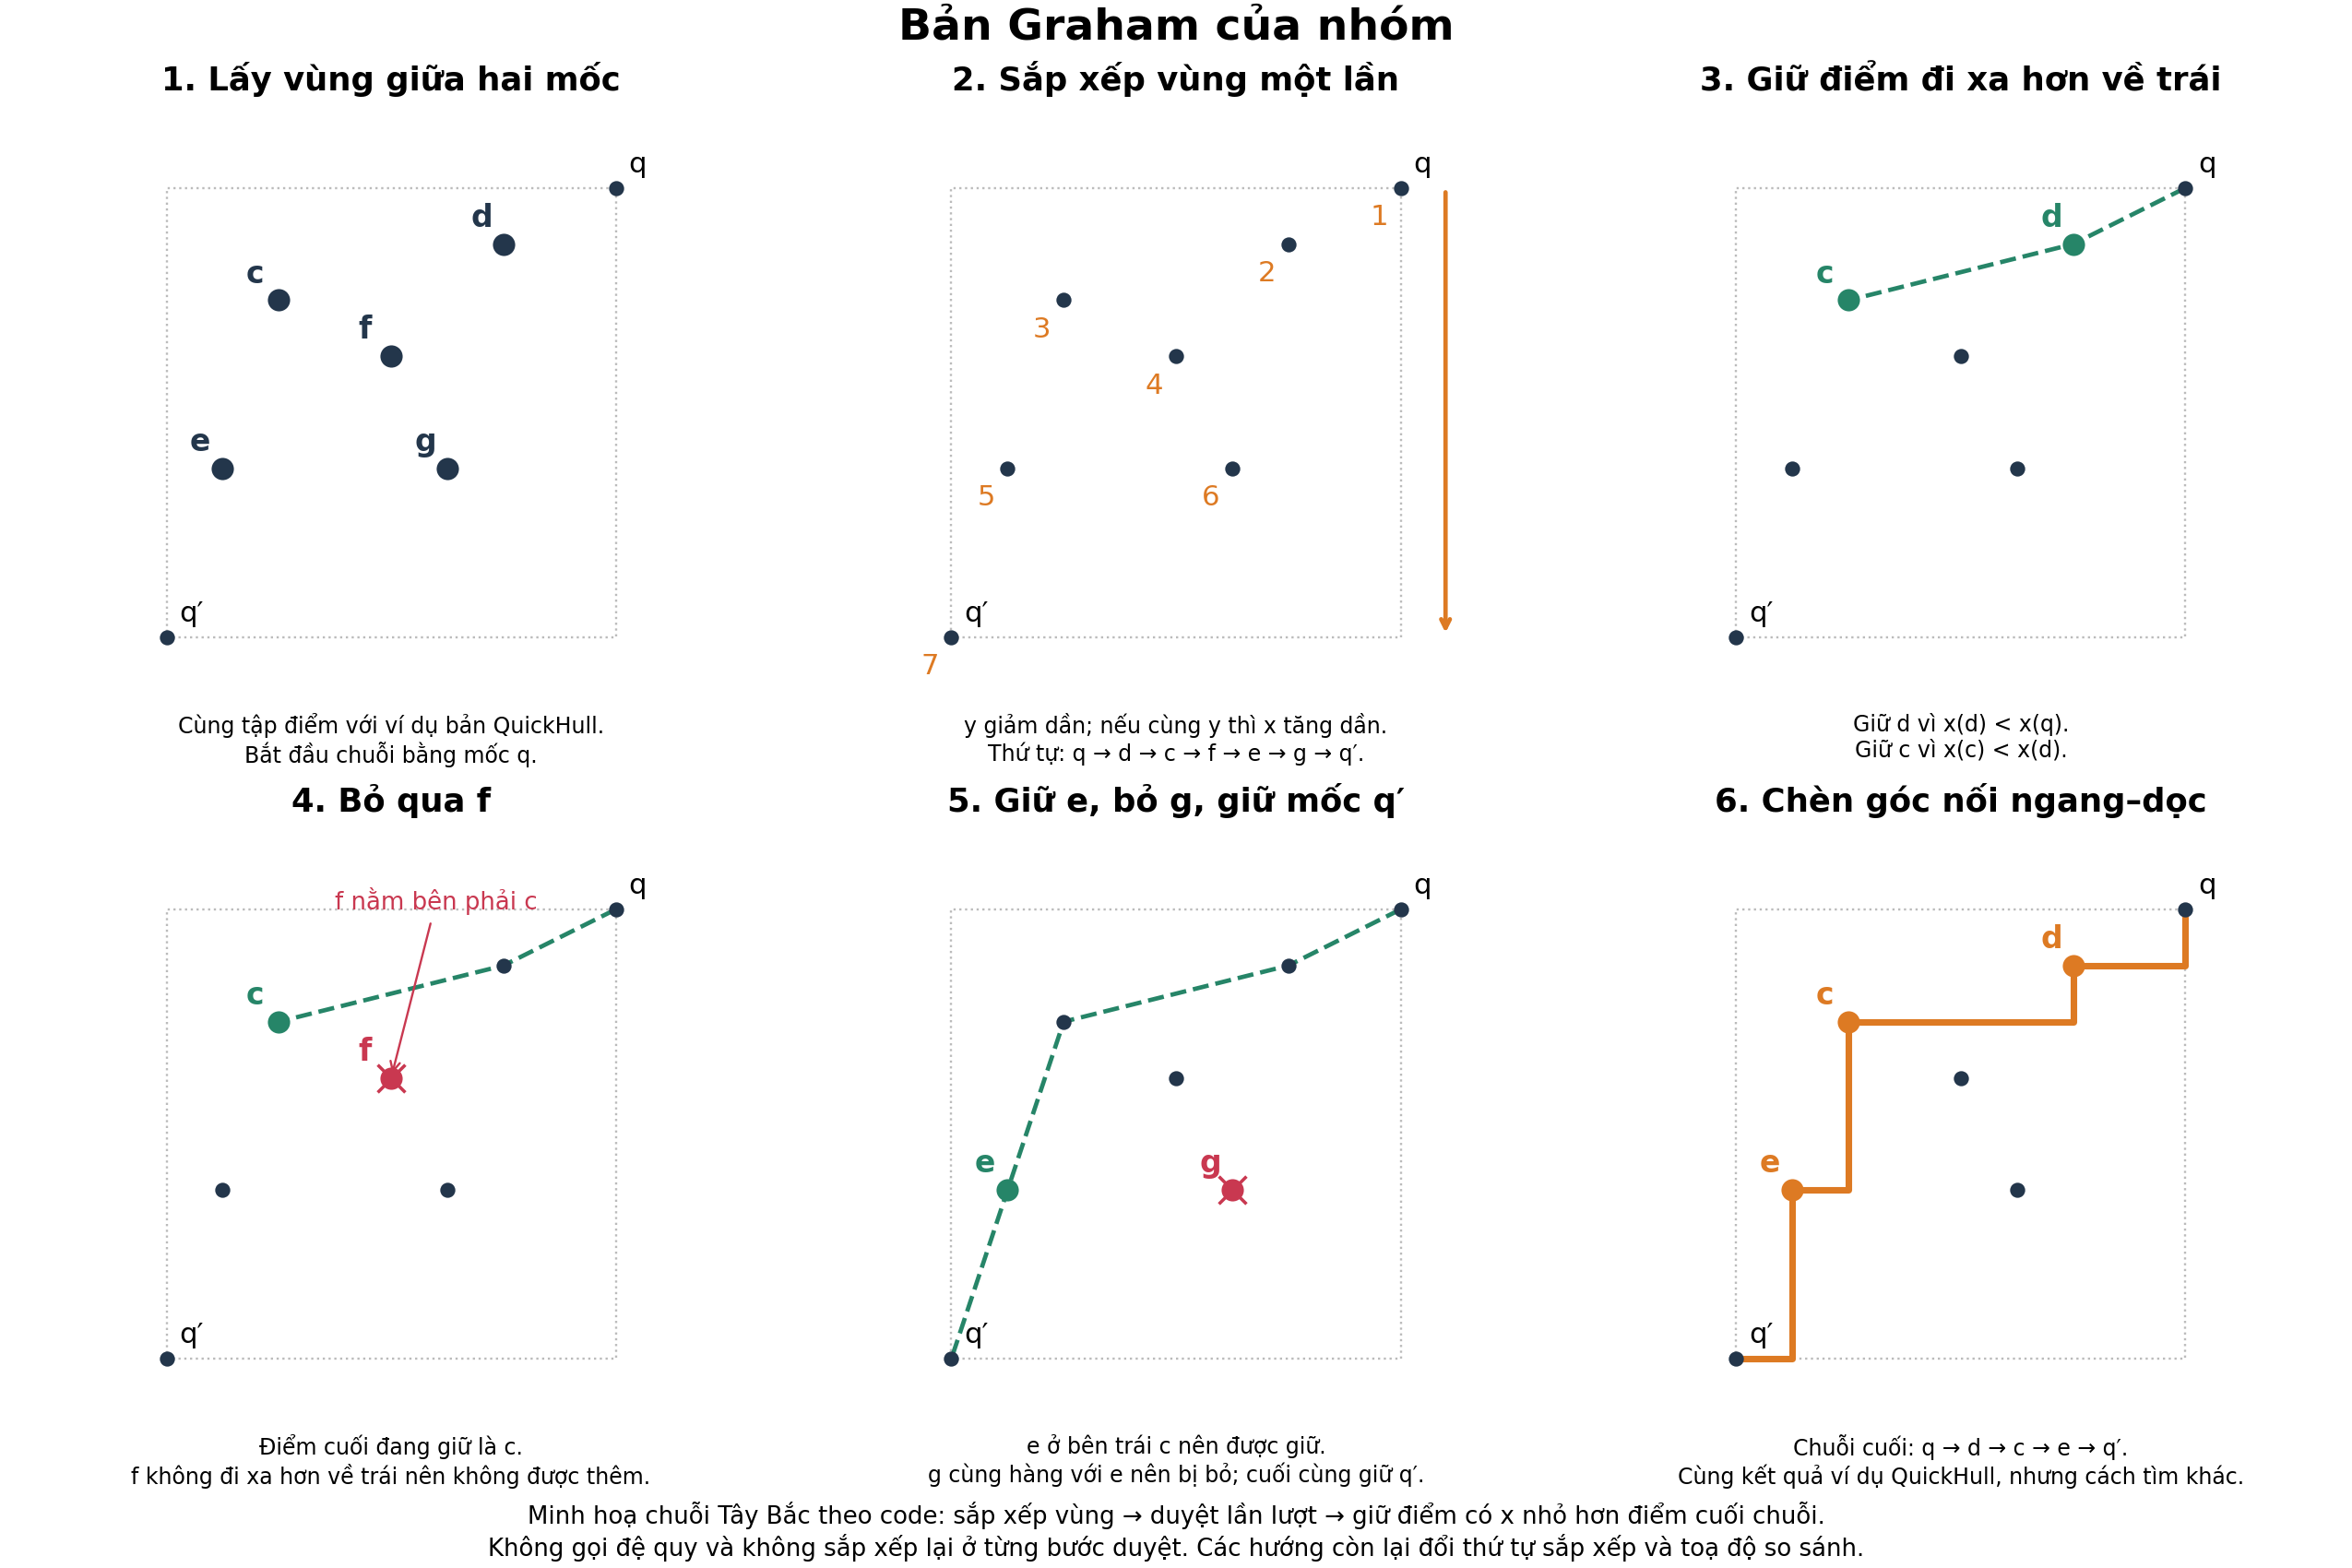
\includegraphics[width=\linewidth]{ograham_group_steps.png}
\caption[Minh hoạ bản Graham]{Các bước tìm chuỗi Tây Bắc theo bản Graham của nhóm. Duyệt từ cao xuống thấp, giữ $d,c,e$ vì chúng lần lượt đi xa hơn về trái; bỏ $f$ vì nằm bên phải $c$ và bỏ $g$ vì không nằm bên trái $e$. Sau khi duyệt và chèn các góc nối, thu được cùng chuỗi như ví dụ bản QuickHull. Hình chỉ minh hoạ một chuỗi biên.}
\label{fig:ograham_steps}
\end{figure}

\begin{algorithm}[H]
\SetAlgoLined
\LinesNumbered
\caption{Bản Graham (cài đặt của nhóm)}
\label{alg:ograham}
\KwIn{Tập điểm $P$, $|P|=n$}
\KwOut{Dãy đỉnh của bao lồi trực giao liên thông, theo thứ tự quanh biên}
Tìm $x_{\min},x_{\max},y_{\min},y_{\max}$ và các điểm mốc\;
$H\gets []$\;
\ForEach{chuỗi $k\in\{\text{Tây Bắc},\text{Tây Nam},\text{Đông Nam},\text{Đông Bắc}\}$}{
  $(s,e)\gets$ điểm mốc đầu và cuối của chuỗi $k$\;
  $R\gets\{p\in P:p\in\operatorname{Rect}(s,e)\}$\;
  Sắp xếp $R$ theo khoá của chuỗi $k$ \tcp*{Tây Bắc: $y$ giảm dần, $x$ tăng dần}
  $C\gets [s]$\;
  \ForEach{$p\in R$ theo thứ tự đã sắp}{
    \If{$p$ vượt điểm cuối của $C$ theo hướng quét của chuỗi $k$}{
      Thêm $p$ vào cuối $C$ \tcp*{Tây Bắc: $p_x<\operatorname{last}(C)_x$}
    }
  }
  Nối dãy $C$ vào cuối $H$\;
}
Với mỗi cặp đỉnh liên tiếp của $H$ khác nhau ở cả hai toạ độ, chèn một đỉnh góc $90^\circ$\;
\Return $H$\;
\end{algorithm}

\begin{table}[H]
\centering
\caption{Khoá sắp xếp và hướng quét của bốn chuỗi}
\label{tab:scan_keys}
\begin{tabular}{lll}
\toprule
Chuỗi & Khoá sắp xếp & Điểm được giữ khi \\
\midrule
Tây Bắc & $y$ giảm dần, rồi $x$ tăng dần & $x$ nhỏ hơn điểm cuối của chuỗi \\
Tây Nam & $x$ tăng dần, rồi $y$ tăng dần & $y$ nhỏ hơn điểm cuối của chuỗi \\
Đông Nam & $y$ tăng dần, rồi $x$ giảm dần & $x$ lớn hơn điểm cuối của chuỗi \\
Đông Bắc & $x$ giảm dần, rồi $y$ giảm dần & $y$ lớn hơn điểm cuối của chuỗi \\
\bottomrule
\end{tabular}
\end{table}


% =====================================================================
\section{Các công trình liên quan}
\label{sec:related}

Phan Thanh An, Phong Thi Thu Huyen và Nguyen Thi Le~\cite{an2021ograham} đề xuất O-Graham để tìm bao lồi trực giao liên thông bằng cách sắp xếp và quét các điểm. Nghiên cứu này là cơ sở tham khảo cho bản Graham của đồ án.

Nguyen Kieu Linh, Phan Thanh An và Tran Van Hoai~\cite{nguyen2022quickhull} đề xuất O-Quickhull, vận dụng ý tưởng chia để trị để tìm các điểm cực trị của bao. Đồ án tham khảo hướng tiếp cận đệ quy này, nhưng bản cài đặt của nhóm chọn điểm theo toạ độ, khác với cách chọn điểm của thuật toán gốc.

Nguyen Kieu Linh~\cite{linh2025parallel} tiếp tục nghiên cứu cách dựng bao hiệu quả cho tập điểm lớn, kết hợp loại bớt điểm không cần xét và xử lý song song. Đồ án chỉ tham khảo hướng phát triển này, chưa cài đặt phương pháp của bài báo.

Từ các nghiên cứu trên, đồ án tập trung ứng dụng bao lồi trực giao để biểu diễn vùng phương tiện. Các phép so sánh tốc độ trong báo cáo chỉ áp dụng cho hai bản cài đặt của nhóm, không phải đánh giá lại hiệu năng của các thuật toán gốc.

% =====================================================================
\section{Theo vết trên video bằng ByteTrack}
\label{sec:tracker}

Theo vết là ghép các phát hiện của cùng một xe qua nhiều khung hình để duy trì một mã định danh (ID). Đồ án sử dụng ByteTrack~\cite{zhang2022bytetrack} có sẵn trong thư viện Ultralytics~\cite{yolo11}, thông qua lệnh \texttt{model.track()} với cấu hình \texttt{bytetrack.yaml}; không tự xây dựng bộ theo vết.

ByteTrack ước lượng vị trí tiếp theo và ghép các hộp dựa trên mức chồng lấp. Các phát hiện có độ tin cậy cao được ghép trước; phát hiện có độ tin cậy thấp vẫn có thể được dùng để nối lại vết đang có. Trong đồ án, tracking chỉ hỗ trợ gắn ID cho phần minh hoạ video, không phải nội dung nghiên cứu chính và không tham gia các phép đánh giá trên ảnh.

% =====================================================================
\section{Độ đo đánh giá}
\label{sec:metrics}

Phần này giải thích các chỉ số dùng trong báo cáo. Các chỉ số đều có giá trị từ 0 đến 1 (hoặc 0\% đến 100\%), càng cao càng tốt.

\paragraph{IoU: hai vùng trùng nhau bao nhiêu.} IoU (Intersection over Union) lấy phần chung của hai vùng chia cho toàn bộ phần chúng phủ.
Với vùng dự đoán $A$ và vùng nhãn chuẩn $B$, tính trên điểm ảnh:
\begin{equation}
  \operatorname{IoU}(A, B) = \frac{|A\cap B|}{|A\cup B|}.
\end{equation}
IoU bằng 1 khi hai vùng trùng khít, bằng 0 khi không chồng lên nhau. Ví dụ, phần chung 80 điểm ảnh và phần phủ 100 điểm ảnh cho IoU bằng 0,8.

\paragraph{Đúng, sai và bỏ sót.} Mỗi dự đoán của mô hình có một \emph{độ tin cậy}, cho biết mô hình chắc chắn đến đâu; dự đoán dưới ngưỡng đã chọn bị bỏ qua.
Một dự đoán được tính là đúng nếu cùng lớp với một nhãn và có IoU với nhãn đó từ 0,5 trở lên; mỗi nhãn chỉ được ghép với một dự đoán, ưu tiên dự đoán có độ tin cậy cao hơn. Trong đánh giá phát hiện đối tượng, báo cáo sử dụng ba loại kết quả TP, FP và FN:
\begin{itemize}
  \item \textbf{TP} (true positive): dự đoán đúng;
  \item \textbf{FP} (false positive): dự đoán sai, tức báo có xe nhưng không ghép được với nhãn nào;
  \item \textbf{FN} (false negative): bỏ sót, tức có nhãn xe nhưng không dự đoán nào ghép được.
\end{itemize}

\paragraph{Precision, Recall và F1.} \emph{Precision} trả lời: trong các xe mô hình báo, bao nhiêu phần là đúng? \emph{Recall} trả lời: trong các xe thật, mô hình tìm được bao nhiêu phần?
Hai chỉ số này thường đánh đổi nhau: báo nhiều hơn thì ít bỏ sót hơn nhưng dễ báo sai hơn. \emph{F1} gộp cả hai thành một số, và chỉ cao khi cả hai cùng cao.
\begin{equation}
  \mathrm{Precision} = \frac{\mathrm{TP}}{\mathrm{TP}+\mathrm{FP}},\qquad
  \mathrm{Recall} = \frac{\mathrm{TP}}{\mathrm{TP}+\mathrm{FN}},\qquad
  F_1 = \frac{2\cdot\mathrm{Precision}\cdot\mathrm{Recall}}{\mathrm{Precision}+\mathrm{Recall}}.
\end{equation}

\paragraph{AP, mAP50 và mAP50--95.} Precision, Recall và F1 phụ thuộc vào một ngưỡng độ tin cậy cố định. \emph{AP} (Average Precision) đánh giá mô hình trên mọi ngưỡng:
nó là diện tích dưới đường cong Precision--Recall của một lớp xe~\cite{everingham2010voc,padilla2021metrics}, nên cao khi mô hình tìm được nhiều xe mà vẫn ít báo sai.
\emph{mAP} (mean AP) là trung bình AP của các lớp xe.
\begin{itemize}
  \item \textbf{mAP50} dùng ngưỡng IoU 0,5: vùng dự đoán chỉ cần khớp vừa phải với nhãn là được tính đúng.
  \item \textbf{mAP50--95} lấy trung bình trên 10 ngưỡng IoU từ 0,50 đến 0,95: ngưỡng càng cao thì vùng càng phải khớp sát, nên chỉ số này khắt khe hơn và phản ánh rõ độ sát của vùng.
\end{itemize}
Đồ án lấy giá trị Precision tại 101 mức Recall cách đều để tính AP theo kiểu COCO~\cite{padilla2021metrics} bằng bộ tính tự viết, không phải công cụ COCOeval chính thức, nên số liệu chỉ dùng để so sánh nội bộ.

\chapter{Thiết kế và cài đặt hệ thống}
\label{chap:design}

\section{Kiến trúc tổng thể}

Hệ thống được tổ chức thành một chuỗi xử lý tuần tự cho từng ảnh hoặc từng khung hình video
(Hình~\ref{fig:pipeline}). Trên video, thư viện Ultralytics kết hợp YOLO11-seg với ByteTrack để trả về hộp, lớp, độ tin cậy, ID và mặt nạ của từng xe. Phần dựng bao chỉ nhận tập điểm biên, nên có thể dùng với mô hình khác nếu mô hình đó cũng cung cấp mặt nạ đối tượng.

\begin{figure}[H]
\centering
\begin{tikzpicture}[grp/.style={draw, dashed, rounded corners, inner sep=5pt}]
  \node (in)   [blk] at (0,0)      {Ảnh / khung hình video};
  \node (yolo) [bb]  at (0,-1.3)   {YOLO11-seg (large)\\ lọc 4 lớp, NMS};
  \node (det)  [bb]  at (0,-2.6)   {Hộp, lớp, độ tin cậy\\ + mặt nạ từng đối tượng};
  % Chế độ video
  \node (trk)  [nk]  at (-3.2,-4.5) {ByteTrack có sẵn:\\ chỉ giữ xe có ID};
  \node (pv)   [nk]  at (-3.2,-5.9) {Đường biên mặt nạ\\ $\rightarrow$ tập điểm $P$\\ (thiếu mặt nạ: vẽ hộp)};
  \node (hv)   [nk]  at (-3.2,-7.4) {Dựng bao bằng\\ hai bản cài đặt};
  \node (ov)   [hd]  at (-3.2,-8.8) {Video có ID + bao;\\ CSV đặc trưng};
  % Chế độ đánh giá
  \node (pe)   [nk]  at (3.2,-4.5)  {Mọi dự đoán trên ảnh có nhãn\\ (không theo vết)};
  \node (he)   [nk]  at (3.2,-5.9)  {Đường biên mặt nạ $\rightarrow$ bao\\ trực giao, bao lồi thường};
  \node (ge)   [nk]  at (3.2,-7.4)  {So từng đầu ra\\ với nhãn chuẩn};
  \node (oe)   [hd]  at (3.2,-8.8)  {Số liệu, biểu đồ,\\ ảnh đối chiếu};
  \draw [arrow] (in) -- (yolo);
  \draw [arrow] (yolo) -- (det);
  \draw [arrow] (det.south) -- (trk.north);
  \draw [arrow] (det.south) -- (pe.north);
  \draw [arrow] (trk) -- (pv);
  \draw [arrow] (pv) -- (hv);
  \draw [arrow] (hv) -- (ov);
  \draw [arrow] (pe) -- (he);
  \draw [arrow] (he) -- (ge);
  \draw [arrow] (ge) -- (oe);
  \begin{scope}[on background layer]
    \node [grp, fit=(trk)(ov), label={[font=\small\bfseries]below:Chế độ video}] {};
    \node [grp, fit=(pe)(oe), label={[font=\small\bfseries]below:Chế độ đánh giá}] {};
  \end{scope}
\end{tikzpicture}
\caption{Sơ đồ hai chế độ chạy của hệ thống}
\label{fig:pipeline}
\end{figure}

Hệ thống có hai chế độ chạy:
\begin{enumerate}
  \item \textbf{Chế độ video}: gọi \texttt{model.track()} để chạy YOLO11-seg cùng ByteTrack, rồi chỉ dựng bao cho các đối tượng
        đã có ID. Đối tượng thiếu mặt nạ được vẽ bằng hộp. Kết quả được vẽ ra hai video riêng và đặc trưng hình học của từng đối tượng được ghi ra CSV.
  \item \textbf{Chế độ đánh giá}: chạy trên tập ảnh có nhãn polygon chuẩn, không qua bộ theo vết. Sáu loại đầu ra (hộp, vùng hình chữ nhật, bao lồi thường, mặt nạ YOLO, hai bản cài đặt bao trực giao)
        được so với nhãn để xuất số liệu, biểu đồ, ảnh đối chiếu.
\end{enumerate}
Do chế độ video chỉ dựng bao cho các đối tượng có ID, số liệu trên ảnh không xác nhận trực tiếp chất lượng của toàn bộ đầu ra video.

\section{Hai bản cài đặt dựng bao}
\label{sec:impl_hull}

Hai bản cài đặt đều làm việc với tối đa tám điểm mốc và bốn chuỗi bậc thang ở mục~\ref{sec:staircase}.
Đây là mã của nhóm, không phải mã của các tác giả bài báo.

\subsection{So sánh hai bản cài đặt}

Bảng~\ref{tab:algo_compare} so sánh hai bản cài đặt của nhóm. Bản QuickHull sắp xếp lại tập điểm ở mỗi lần gọi và có thể cần nhiều lần gọi khi số điểm trên biên lớn, nên có cận xấu nhất $O(n^2\log n)$; bản Graham có cận $O(n\log n)$.



\begin{table}[H]
\centering
\caption{So sánh hai bản cài đặt của nhóm}
\label{tab:algo_compare}
\begin{tabular}{>{\raggedright\arraybackslash}p{4.2cm} >{\raggedright\arraybackslash}p{5.2cm} >{\raggedright\arraybackslash}p{5.2cm}}
\toprule
\textbf{Tiêu chí} & \textbf{Bản QuickHull} & \textbf{Bản Graham} \\
\midrule
Chiến lược & Đệ quy một nhánh & Sắp xếp rồi quét một lượt \\
Độ phức tạp xấu nhất & $O(n^2\log n)$ & $O(n\log n)$ \\
Bộ nhớ phụ xấu nhất & $O(n^2)$ (danh sách điểm ở mỗi tầng đệ quy) & $O(n)$ \\
Kết quả trên dữ liệu thử & \multicolumn{2}{c}{Cùng một vùng bao trên dữ liệu thử} \\
\bottomrule
\end{tabular}
\end{table}

Hai bản cài đặt chưa bảo đảm bao tối tiểu trên mọi đầu vào; chẳng hạn, với hai điểm chéo nhau, mã trả về hình chữ nhật thay vì đường bậc thang.

\section{Chi tiết cài đặt}

Hệ thống được viết bằng Python. Để hai bản cài đặt được so sánh công bằng, cả hai đều được gọi qua cùng một hàm chuẩn hoá:
\begin{enumerate}
  \item Ép toạ độ về số nguyên và loại các điểm trùng nhau.
  \item Nếu còn ít hơn 2 điểm phân biệt, trả về chính các điểm đó. Với 2 hoặc 3 điểm, hai bản cài đặt dùng chung nhánh O-Graham để mọi cạnh vẫn song song với trục.
  \item Gọi bản QuickHull hoặc bản Graham.
  \item Thêm lại điểm đầu vào cuối dãy đỉnh để khép kín đa giác.
\end{enumerate}
Sau đó, hệ thống tính diện tích, chu vi, tỉ lệ lấp đầy so với hộp và số đỉnh của bao.
Bộ đếm thời gian chỉ bao quanh bước dựng bao, không tính inference YOLO, vẽ hay ghi tệp.
Trên video, ID được lấy từ \texttt{result.boxes.id}; hộp, lớp, độ tin cậy và mặt nạ được đọc theo cùng chỉ số trong kết quả do Ultralytics trả về. Nhờ đó, bao được dựng từ mặt nạ tương ứng với ID đang hiển thị.

Nhãn chuẩn ở định dạng YOLO polygon (đa giác có toạ độ được chia cho chiều rộng và chiều cao ảnh để đưa về khoảng từ 0 đến 1): mỗi polygon được nhân với kích thước ảnh, làm tròn rồi tô thành mặt nạ tại độ phân giải gốc; ảnh có nhãn phương tiện chỉ ở dạng hộp bị loại.

\chapter{Thực nghiệm và đánh giá}
\label{chap:exp}

Chương này lần lượt trả lời ba câu hỏi CH1--CH3 nêu ở mục~\ref{sec:questions}: Thí nghiệm 1 cho CH1, Thí nghiệm 2 cho CH2
và Thí nghiệm 3 cho CH3. Thí nghiệm 3 là trọng tâm vì đo trực tiếp việc thay mặt nạ YOLO bằng bao lồi trực giao.
Chất lượng được đo trên 100 ảnh giao thông Việt Nam có nhãn, với YOLO11-l được chọn ở bước so sánh sơ bộ (mục~\ref{sec:model_select}).
Video không có nhãn nên chỉ dùng để minh hoạ và đo thời gian.

% =====================================================================
\section{Dữ liệu}
\label{sec:data}

Nguồn là bộ \emph{Vietnam Traffic Vehicle Detection} trên Roboflow Universe \cite{roboflowvn} (giấy phép CC BY 4.0):
756 ảnh (601 huấn luyện, 126 kiểm định, 29 kiểm tra), được đưa về kích thước $640\times640$.
Đồ án sử dụng bốn lớp \texttt{car}, \texttt{truck}, \texttt{bus}, \texttt{motorcycle}. Ảnh được trích từ nhiều video camera giao thông.

Bộ đánh giá 100 ảnh được xây dựng từ bộ nguồn theo quy trình:
\begin{enumerate}
  \item Chỉ giữ ảnh mà \emph{mọi} nhãn phương tiện đều là polygon, tức đa giác mô tả đường viền xe; loại ảnh có nhãn chỉ ở dạng hộp và ảnh có nội dung điểm ảnh trùng nhau.
  \item Quan sát từng ảnh để phân nhóm theo mức độ nhìn rõ phương tiện, dựa vào kích thước xe trong ảnh,
        mức che khuất và việc xe bị cắt ở mép ảnh. Đây là nhận định thủ công của nhóm, không phải thang đo độ khó chuẩn hoá;
        số lượng xe trong ảnh không được dùng làm tiêu chí phân nhóm.
  \item Chọn 100 ảnh gồm 70 ảnh được nhóm đánh giá là dễ (xe chính rõ hình dạng, ít che khuất),
        20 ảnh mức trung bình và 10 ảnh được đánh giá là khó (xe nhỏ, bị che khuất nhiều hoặc bị cắt ở mép ảnh).
        Hình dạng nhãn được giữ nguyên.
\end{enumerate}
Kết quả: 100 ảnh, 540 phương tiện: 179 car, 110 truck, 26 bus, 225 motorcycle.
Ảnh lấy từ cả ba phần của bộ nguồn (74 huấn luyện, 20 kiểm định, 6 kiểm tra).

Video minh hoạ do nhóm cung cấp quay cảnh giao thông ban đêm, gồm 1\,647 khung hình ở độ phân giải $1280\times720$. Video không có nhãn chuẩn và chỉ dùng để minh hoạ đầu ra.

% =====================================================================
\section{Cấu hình thực nghiệm}

\begin{table}[H]
\centering
\caption{Cấu hình inference và đánh giá (dùng chung cho mọi thí nghiệm trên ảnh)}
\label{tab:config}
\begin{tabular}{ll}
\toprule
Tham số & Giá trị \\
\midrule
Kích thước ảnh đầu vào (\texttt{imgsz}) & 960 \\
Ngưỡng độ tin cậy cho P/R/F1 & 0,20 \\
Ngưỡng độ tin cậy tối thiểu khi tính AP & 0,001 \\
Số phát hiện tối đa mỗi ảnh & 300 \\
Lớp giữ lại & car, truck, bus, motorcycle \\
\bottomrule
\end{tabular}
\end{table}

Với \texttt{imgsz=960}, ảnh gốc $640\times640$ được phóng lên khi inference.
Đồ án chưa khảo sát ảnh hưởng của kích thước đầu vào đến chất lượng và tốc độ.

Các bảng kết quả so sánh năm cách biểu diễn xe: hộp phát hiện, vùng hình chữ nhật, bao lồi thường, mặt nạ YOLO và bao lồi trực giao.

Hộp phát hiện được so với hộp của nhãn chuẩn. Bốn cách còn lại được so theo phần vùng chồng khớp với mặt nạ nhãn chuẩn. Các vùng bao được dựng từ điểm biên của mặt nạ YOLO.

Hai bản QuickHull và Graham cho cùng vùng bao trên dữ liệu đánh giá, nên bảng chỉ ghi một dòng ``Bao trực giao''.

% =====================================================================
\section{So sánh sơ bộ và chọn mô hình}
\label{sec:model_select}

Trong bảng so sánh, số tham số phản ánh lượng giá trị mà mô hình đã học; GFLOPs là số tỉ phép tính cho một lần xử lý ảnh ở kích thước được ghi trong bảng.

Mặt nạ là đầu vào để dựng bao, nên mặt nạ kém thì bao cũng kém theo. Vì vậy, trước các thí nghiệm, nhóm so sánh kích thước và chất lượng mặt nạ của hai mô hình trên 100 ảnh Việt Nam, rồi chọn một mô hình cho phần còn lại của chương.

\begin{table}[H]
\centering
\caption{So sánh sơ bộ hai mô hình: kích thước và chất lượng mặt nạ trên 100 ảnh Việt Nam (540 nhãn)}
\label{tab:model_select}
\begin{tabular}{lrr}
\toprule
Chỉ số & YOLO11-n & YOLO11-l \\
\midrule
Số tham số & 2,88 triệu & 27,68 triệu \\
Số phép tính (GFLOPs, ảnh $640\times640$) & 9,9 & 132,9 \\
\midrule
Precision & 65,1\% & 74,9\% \\
Recall & 57,8\% & 71,7\% \\
F1 & 61,2\% & 73,2\% \\
mAP50 & 63,5\% & 74,6\% \\
mAP50--95 & 43,8\% & 55,1\% \\
Recall của lớp xe máy & 41,3\% & 65,3\% \\
\bottomrule
\end{tabular}
\end{table}

YOLO11-l có chất lượng mặt nạ cao hơn YOLO11-n ở mọi chỉ số, cách biệt rõ nhất ở recall của lớp xe máy. Đổi lại, mô hình này nặng hơn nhiều, cả về số tham số lẫn số phép tính.
Đồ án ưu tiên chất lượng mặt nạ hơn tốc độ nên chọn YOLO11-l cho toàn bộ các thí nghiệm sau. Đây chỉ là phép so sơ bộ để chọn mô hình, không phải đánh giá đầy đủ hai mô hình.

% =====================================================================
\section{Thí nghiệm 1: Khả năng biểu diễn hình dạng}
\label{sec:exp_shape}

Để tách riêng khả năng biểu diễn khỏi sai số của mô hình, đồ án sử dụng \emph{mặt nạ nhãn chuẩn} của 540 phương tiện Việt Nam,
dựng ba loại vùng bao từ biên của mặt nạ và đo IoU của từng vùng với chính mặt nạ đó.
Bảng~\ref{tab:shape} cho thấy bao lồi trực giao khớp với hình dạng xe tốt hơn bao lồi thông thường và tốt hơn nhiều so với hình chữ nhật bao, rõ nhất ở xe máy. Phép đo này dựng bao từ chính mặt nạ nhãn, nên chỉ cho biết khả năng biểu diễn khi đầu vào đã đúng,
không phải chất lượng của cả chuỗi xử lý; phần đó ở Thí nghiệm 3.

\begin{table}[H]
\centering
\caption{IoU trung bình giữa vùng bao và mặt nạ nhãn chuẩn (bộ Việt Nam, 540 phương tiện)}
\label{tab:shape}
\begin{tabular}{lrrrr}
\toprule
Lớp & Số xe & Hình chữ nhật & Bao lồi & \textbf{Bao lồi trực giao} \\
\midrule
car        & 179 & 74,2\% & 91,6\% & \textbf{97,0\%} \\
truck      & 110 & 74,5\% & 89,4\% & \textbf{95,8\%} \\
bus        &  26 & 71,4\% & 87,5\% & \textbf{94,5\%} \\
motorcycle & 225 & 64,6\% & 84,3\% & \textbf{92,6\%} \\
\midrule
Tất cả     & 540 & 70,1\% & 87,9\% & \textbf{94,8\%} \\
\bottomrule
\end{tabular}
\end{table}

Hình~\ref{fig:real_vehicle} minh hoạ trên nhãn của một xe máy. Nhãn này không bao trọn người lái, nên hình chỉ phản ánh độ khớp về hình học với nhãn đã cho.

\begin{figure}[H]
\centering
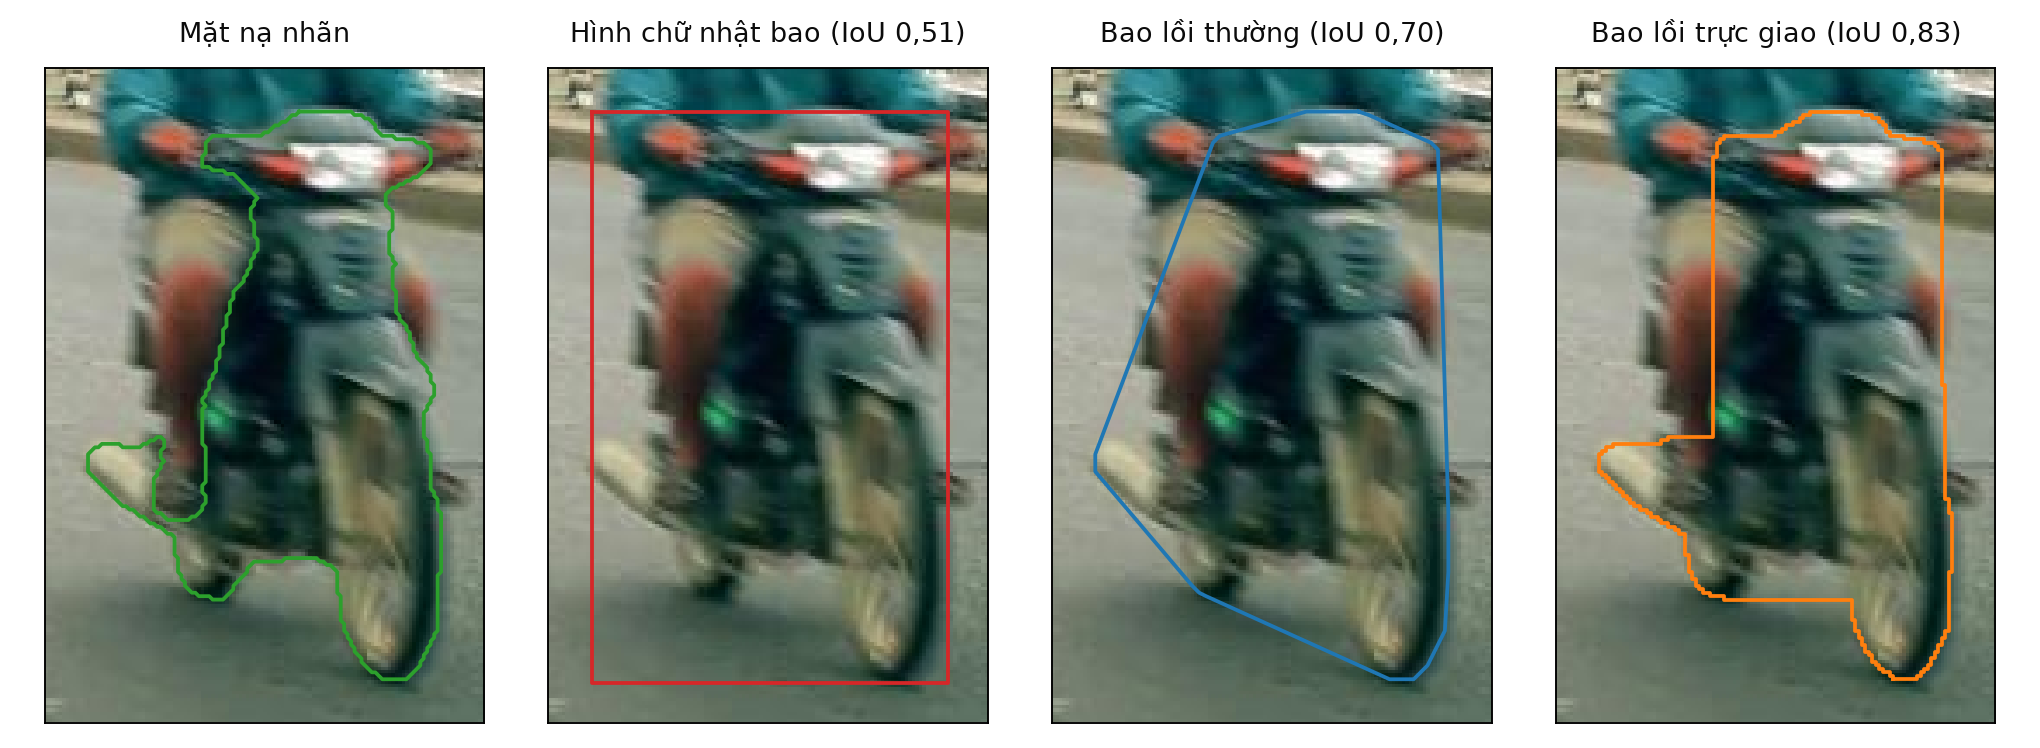
\includegraphics[width=\textwidth]{hull_real_vehicle.png}
\caption{Bốn cách biểu diễn vùng của cùng một xe máy trong bộ dữ liệu Việt Nam}
\label{fig:real_vehicle}
\end{figure}

% =====================================================================
\section{Thí nghiệm 2: Tốc độ hai bản cài đặt}
\label{sec:exp_speed}

Chỉ đo thời gian dựng bao (gồm các bước đưa đầu vào và đầu ra về cùng quy ước cho cả hai bản cài đặt) với hai bản cài đặt ở mục~\ref{sec:impl_hull}. Kết quả chỉ dùng để so sánh hai bản cài đặt của nhóm. Trung vị là giá trị ở giữa khi xếp các kết quả từ nhỏ đến lớn (nếu có hai giá trị ở giữa thì lấy trung bình của chúng). Phép đo sử dụng hai loại đầu vào:
\begin{itemize}
  \item Tổng hợp: $n \in \{100, 500, 1\,000, 2\,000, 5\,000, 10\,000\}$ điểm nguyên trong vùng $4000\times4000$,
        theo hai phân bố: \emph{đều} trong hình vuông (bao có ít đỉnh) và \emph{trên đường tròn} (hầu hết các điểm
        đều là đỉnh bao, trường hợp xấu).
  \item Đường biên thật: biên đầy đủ của 540 mặt nạ nhãn Việt Nam (12--1\,768 điểm, trung vị 165),
        mỗi xe lấy trung vị 5 lượt.
\end{itemize}

Hình~\ref{fig:synthetic_distributions} minh hoạ hai kiểu dữ liệu tổng hợp: phân bố đều là các điểm được lấy ngẫu nhiên khắp vùng vuông, còn dữ liệu đường tròn chỉ có điểm trên đường viền tròn.

\begin{figure}[H]
\centering
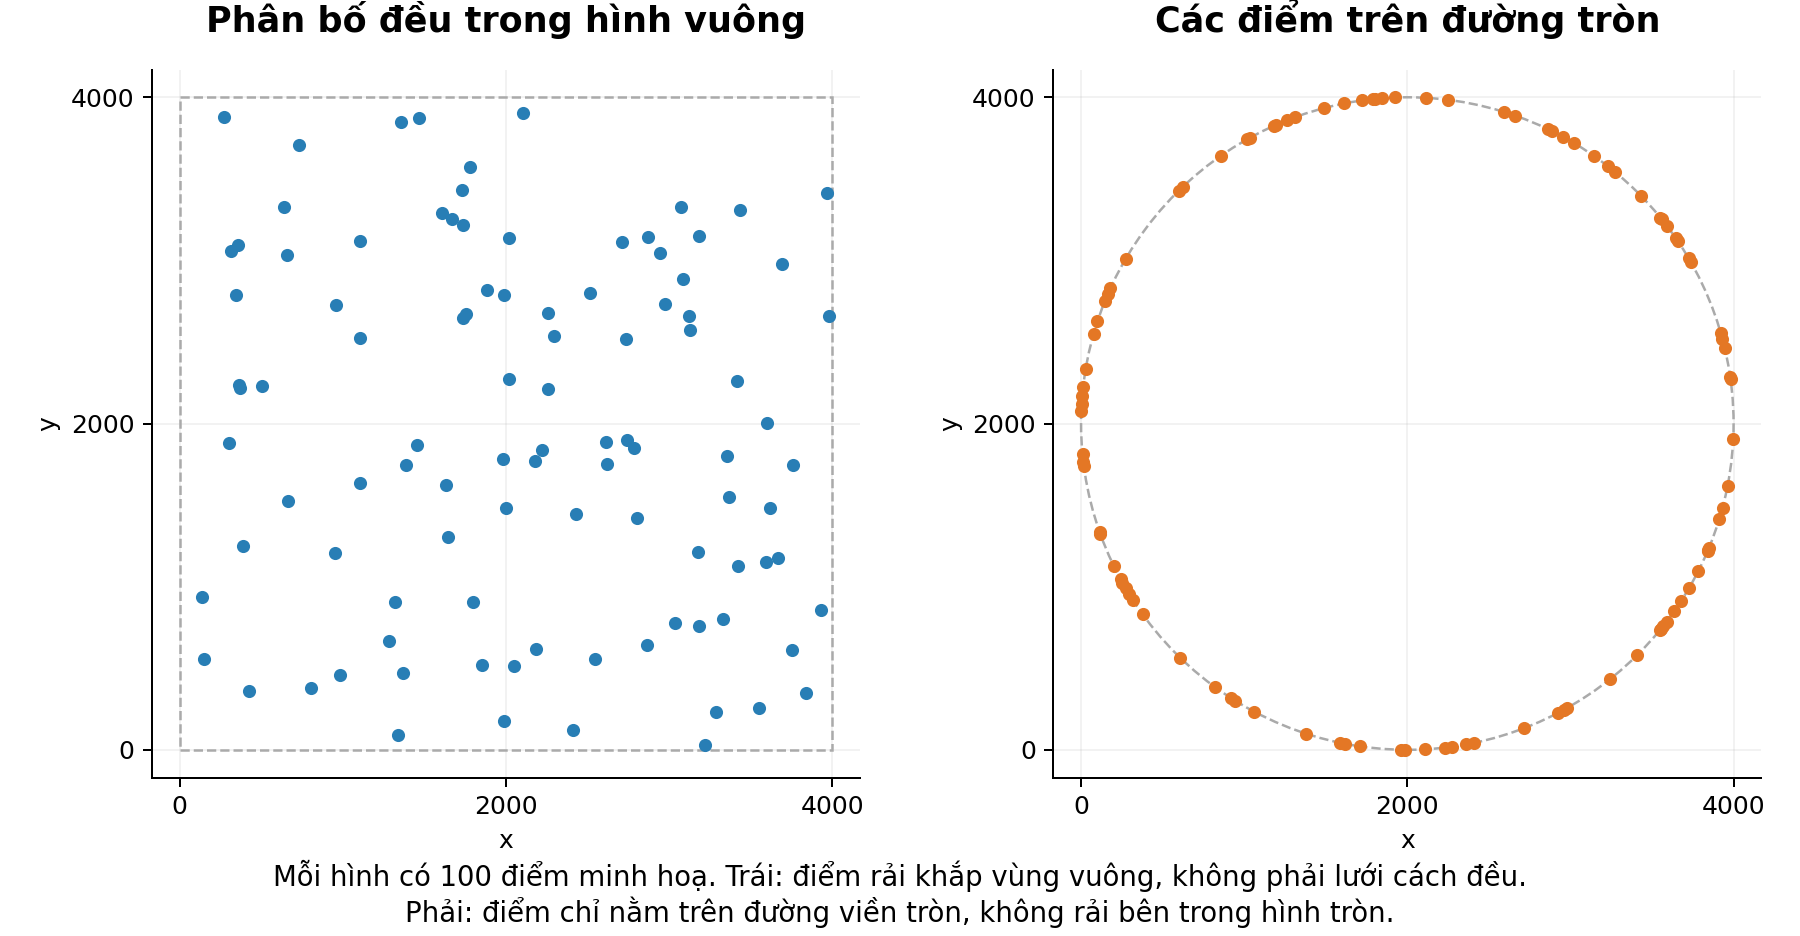
\includegraphics[width=\linewidth]{synthetic_point_distributions.png}
\caption{Hai kiểu dữ liệu dùng để đo tốc độ, minh hoạ với 100 điểm mỗi kiểu trong vùng $4000\times4000$. Trái: điểm ngẫu nhiên theo phân bố đều trong hình vuông. Phải: điểm có góc ngẫu nhiên nằm trên đường tròn, sau đó làm tròn toạ độ về số nguyên.}
\label{fig:synthetic_distributions}
\end{figure}



\begin{table}[H]
\centering
\caption{Thời gian dựng bao (ms, trung vị 30 lượt) trên tập điểm tổng hợp}
\label{tab:speed_syn}
\begin{tabular}{rrrrr}
\toprule
\multirow{2}{*}{$n$} & \multicolumn{2}{c}{Phân bố đều} & \multicolumn{2}{c}{Trên đường tròn} \\
\cmidrule(lr){2-3}\cmidrule(lr){4-5}
 & Bản QuickHull & Graham & Bản QuickHull & Graham \\
\midrule
100    & 0,27  & 0,29  & 0,65  & 0,32 \\
500    & 1,41  & 1,31  & 9,02  & 1,43 \\
1\,000 & 2,21  & 2,35  & 31,2  & 2,80 \\
2\,000 & 3,79  & 4,59  & 101,7 & 5,54 \\
5\,000 & 9,14  & 11,66 & 404,6 & 12,7 \\
10\,000& 22,5  & 25,8  & 918,9 & 22,8 \\
\bottomrule
\end{tabular}
\end{table}

\begin{table}[H]
\centering
\caption{Thời gian dựng bao trên 540 đường biên xe thật}
\label{tab:speed_real}
\begin{tabular}{lrrr}
\toprule
Bản cài đặt & Trung vị (ms) & Trung bình (ms) & Tổng 540 xe (ms) \\
\midrule
Bản QuickHull & 0,648 & 1,509 & 815 \\
Graham            & \textbf{0,458} & \textbf{0,658} & \textbf{356} \\
\bottomrule
\end{tabular}
\end{table}

\begin{figure}[H]
\centering
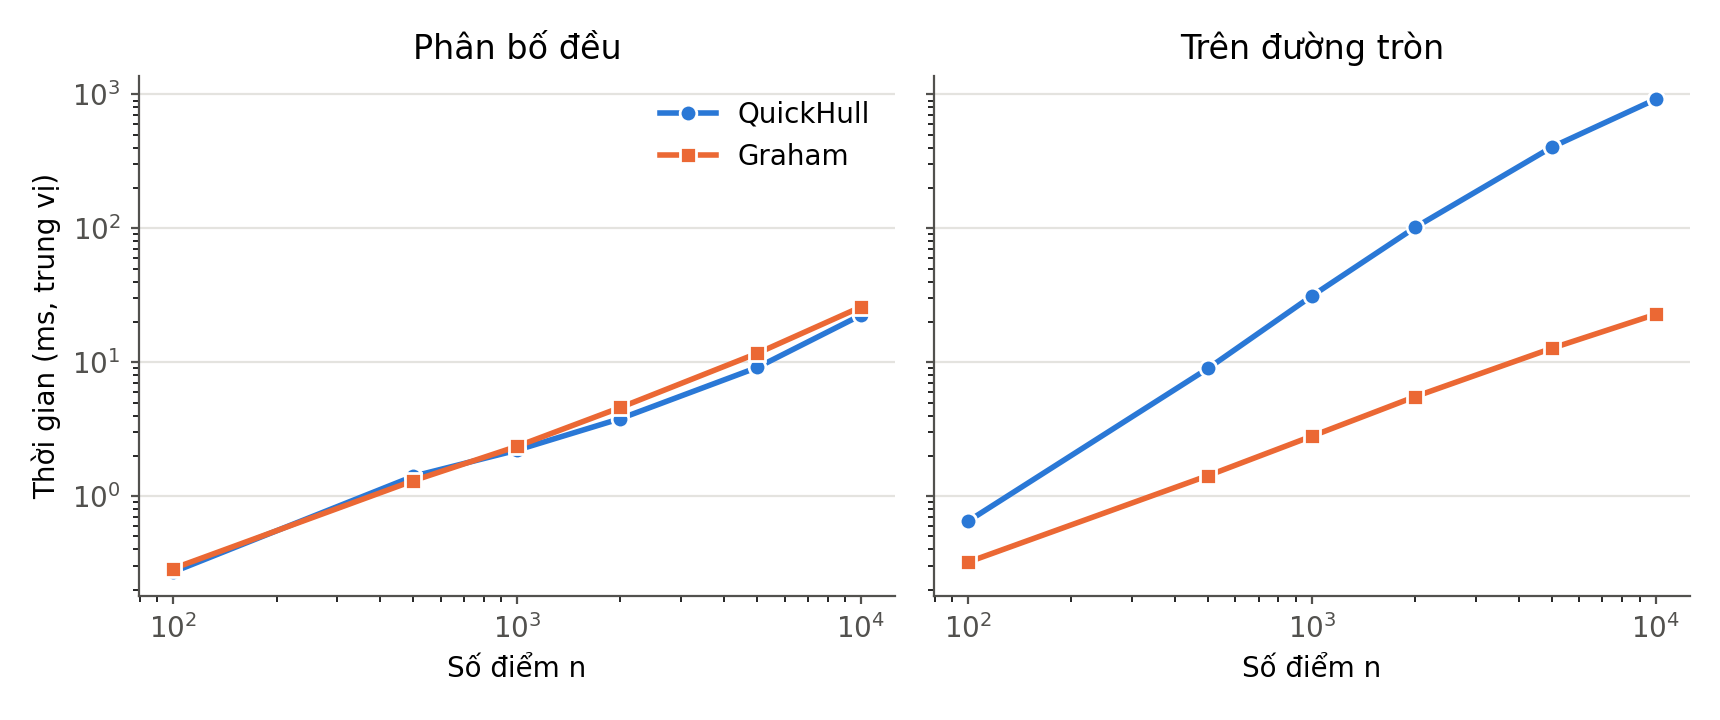
\includegraphics[width=\textwidth]{hull_speed.png}
\caption{Thời gian dựng bao theo số điểm; cả hai trục dùng thang logarit, tức các khoảng cách bằng nhau trên trục biểu diễn cùng một mức tăng theo tỉ lệ. Trái: phân bố đều; phải: trên đường tròn.}
\label{fig:speed}
\end{figure}

Từ các kết quả trên có thể rút ra:
\begin{itemize}
  \item Với phân bố đều, thời gian hai bản cài đặt gần nhau; bản QuickHull nhanh hơn một chút ở $n$ lớn.
  \item Với điểm trên đường tròn, thời gian của bản QuickHull tăng nhanh hơn nhiều so với mức tăng của số điểm, phù hợp với cận xấu nhất $O(n^2\log n)$ nêu trong Bảng~\ref{tab:algo_compare}.
        Thời gian O-Graham vẫn tăng gần theo tỉ lệ với số điểm nên nhanh hơn rõ rệt khi $n$ lớn.
  \item Trên đường biên xe thật, bản Graham có thời gian trung vị và trung bình thấp hơn bản QuickHull.
  \item Mỗi cấu hình tổng hợp dùng một tập điểm cố định, được tạo với cùng giá trị khởi tạo bộ sinh số ngẫu nhiên (hạt giống), nên 30 lượt đo phản ánh biến thiên thời gian trên đầu vào đó, không phải trên nhiều tập điểm.
  \item Hai bản QuickHull và Graham cho cùng vùng bao trên các cấu hình đã thử.
\end{itemize}

% =====================================================================
\section{Thí nghiệm 3: Thay mặt nạ YOLO bằng bao lồi trực giao}
\label{sec:exp_quality}

Thí nghiệm này dùng YOLO11-l trên bộ Việt Nam, so bốn cách biểu diễn vùng cùng lấy từ một dự đoán: hình chữ nhật, bao lồi thường, bao trực giao và mặt nạ.
Bao được dựng từ chính mặt nạ, nên phép so cho biết việc đơn giản hoá mặt nạ thành bao làm mất bao nhiêu độ khớp với nhãn và đổi lại được gì.
Bao không sửa được xe bị bỏ sót hay sai lớp.

\subsection{Mức giảm chất lượng}

\begin{figure}[H]
\centering
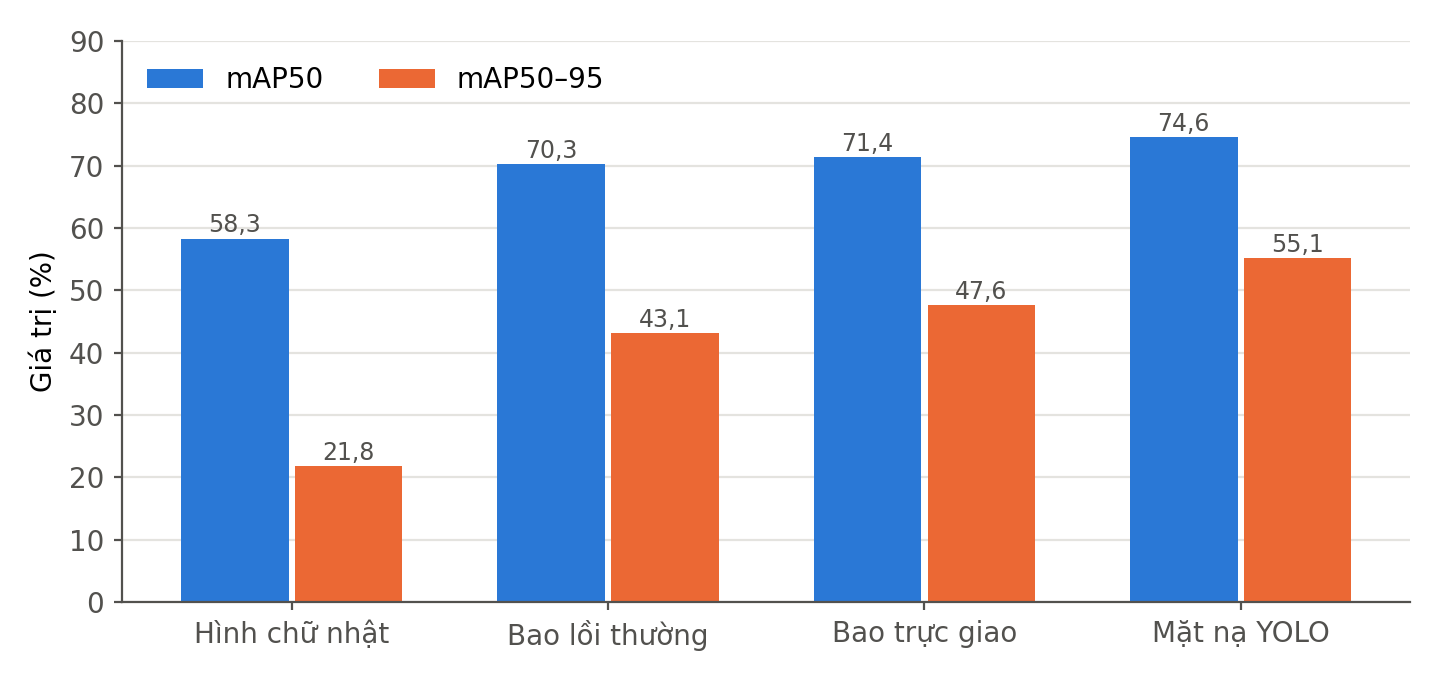
\includegraphics[width=0.85\textwidth]{mask_vs_hull_map.png}
\caption{mAP50 và mAP50--95 của bốn cách biểu diễn vùng (YOLO11-l, bộ Việt Nam; ghép đúng lớp, so với cùng mặt nạ nhãn)}
\label{fig:mask_vs_hull}
\end{figure}

\begin{table}[H]
\centering
\caption{Kết quả trên 100 ảnh Việt Nam, mô hình YOLO11-l (540 nhãn)}
\label{tab:vn_large}
\begin{tabular}{lrrrrr}
\toprule
Đầu ra & Precision & Recall & F1 & mAP50 & mAP50--95 \\
\midrule
Hộp phát hiện & 73,1\% & 70,0\% & 71,5\% & 72,3\% & 56,0\% \\
Vùng hình chữ nhật   & 61,3\% & 58,7\% & 60,0\% & 58,3\% & 21,8\% \\
Bao lồi thường        & 71,0\% & 68,0\% & 69,4\% & 70,3\% & 43,1\% \\
Bao trực giao        & 72,1\% & 69,1\% & 70,6\% & 71,4\% & 47,6\% \\
Mặt nạ YOLO     & 74,9\% & 71,7\% & 73,2\% & 74,6\% & 55,1\% \\
\bottomrule
\end{tabular}
\end{table}

Ý nghĩa các chỉ số được giải thích ở mục~\ref{sec:metrics}. Hàng Hộp phát hiện so hộp với hộp nhãn nên là một phép đo khác, không so trực tiếp được với bốn hàng vùng điểm ảnh.
Hai bản cài đặt bao trực giao cho kết quả trùng nhau ở mọi độ đo. Từ các kết quả này:
\begin{itemize}
  \item So với mặt nạ YOLO, bao giảm nhẹ ở mAP50 và giảm nhiều hơn ở mAP50--95. Nguyên nhân là bao lấp thêm các phần lõm của mặt nạ:
        xe vẫn được nhận ra, nhưng vùng không còn khớp sát như mặt nạ.
  \item So với vùng hình chữ nhật, bao tốt hơn rõ rệt, nhất là ở mAP50--95.
  \item So với bao lồi thường, bao cao hơn nhẹ ở mAP50 và cao hơn rõ hơn ở mAP50--95. Như vậy, kết quả của CH1 cũng đúng trên mặt nạ dự đoán.
\end{itemize}

Mức giảm mAP50--95 từ mặt nạ xuống bao có ở cả bốn lớp xe, không chỉ xe máy, và lớn hơn ở bus (chỉ 26 nhãn) và motorcycle.

\subsection{Ma trận nhầm lẫn}

Ghép không xét lớp cho thấy trong các cặp đã định vị được, YOLO11-l phân loại đúng 92,7\%.
Lỗi nhiều nhất là car $\rightarrow$ truck (12 trường hợp), tiếp theo là truck $\rightarrow$ car (9) và
truck $\rightarrow$ bus (8). Xem trực quan các ca car $\rightarrow$ truck thì chủ yếu là
xe van và xe gầm cao; các ca truck $\rightarrow$ bus chủ yếu là xe tải thùng cao phủ bạt.

\begin{figure}[H]
\centering
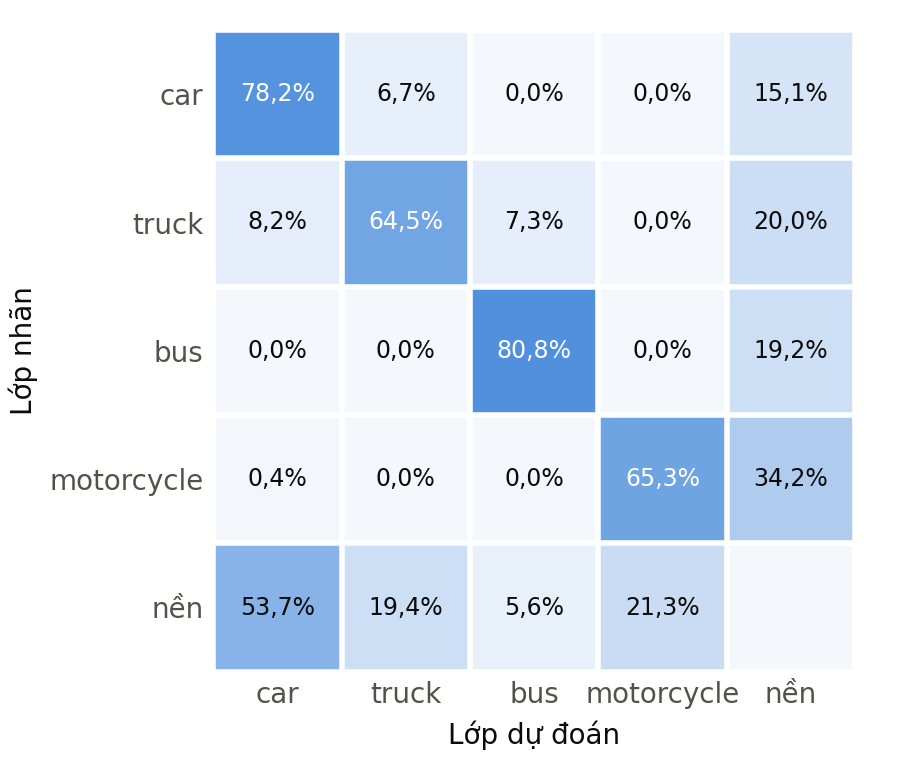
\includegraphics[width=0.62\textwidth]{vn_large_confusion.png}
\caption{Ma trận nhầm lẫn của mặt nạ YOLO (YOLO11-l), chuẩn hoá theo hàng. Hàng ``nền'' là phân bố các dự đoán thừa theo lớp.
}
\label{fig:vn_class}
\end{figure}

\subsection{Độ gọn và tính liên thông của vùng bao}

So với đường biên đã được OpenCV rút gọn, số đỉnh của bao chỉ ít hơn một phần nhỏ, nên độ gọn không phải lợi ích chính.
Lợi ích rõ hơn là về hình học: bao luôn là một vùng liền khối, không lỗ, các cạnh song song với trục, nên diện tích và chu vi tính trực tiếp từ đỉnh,
trong khi khoảng một phần năm mặt nạ bị đứt thành nhiều mảnh. Nối các mảnh cũng có thể làm bao lấp sang vùng không phải xe, như ca giảm nhiều nhất ở Hình~\ref{fig:crops}.

\begin{figure}[H]
\centering
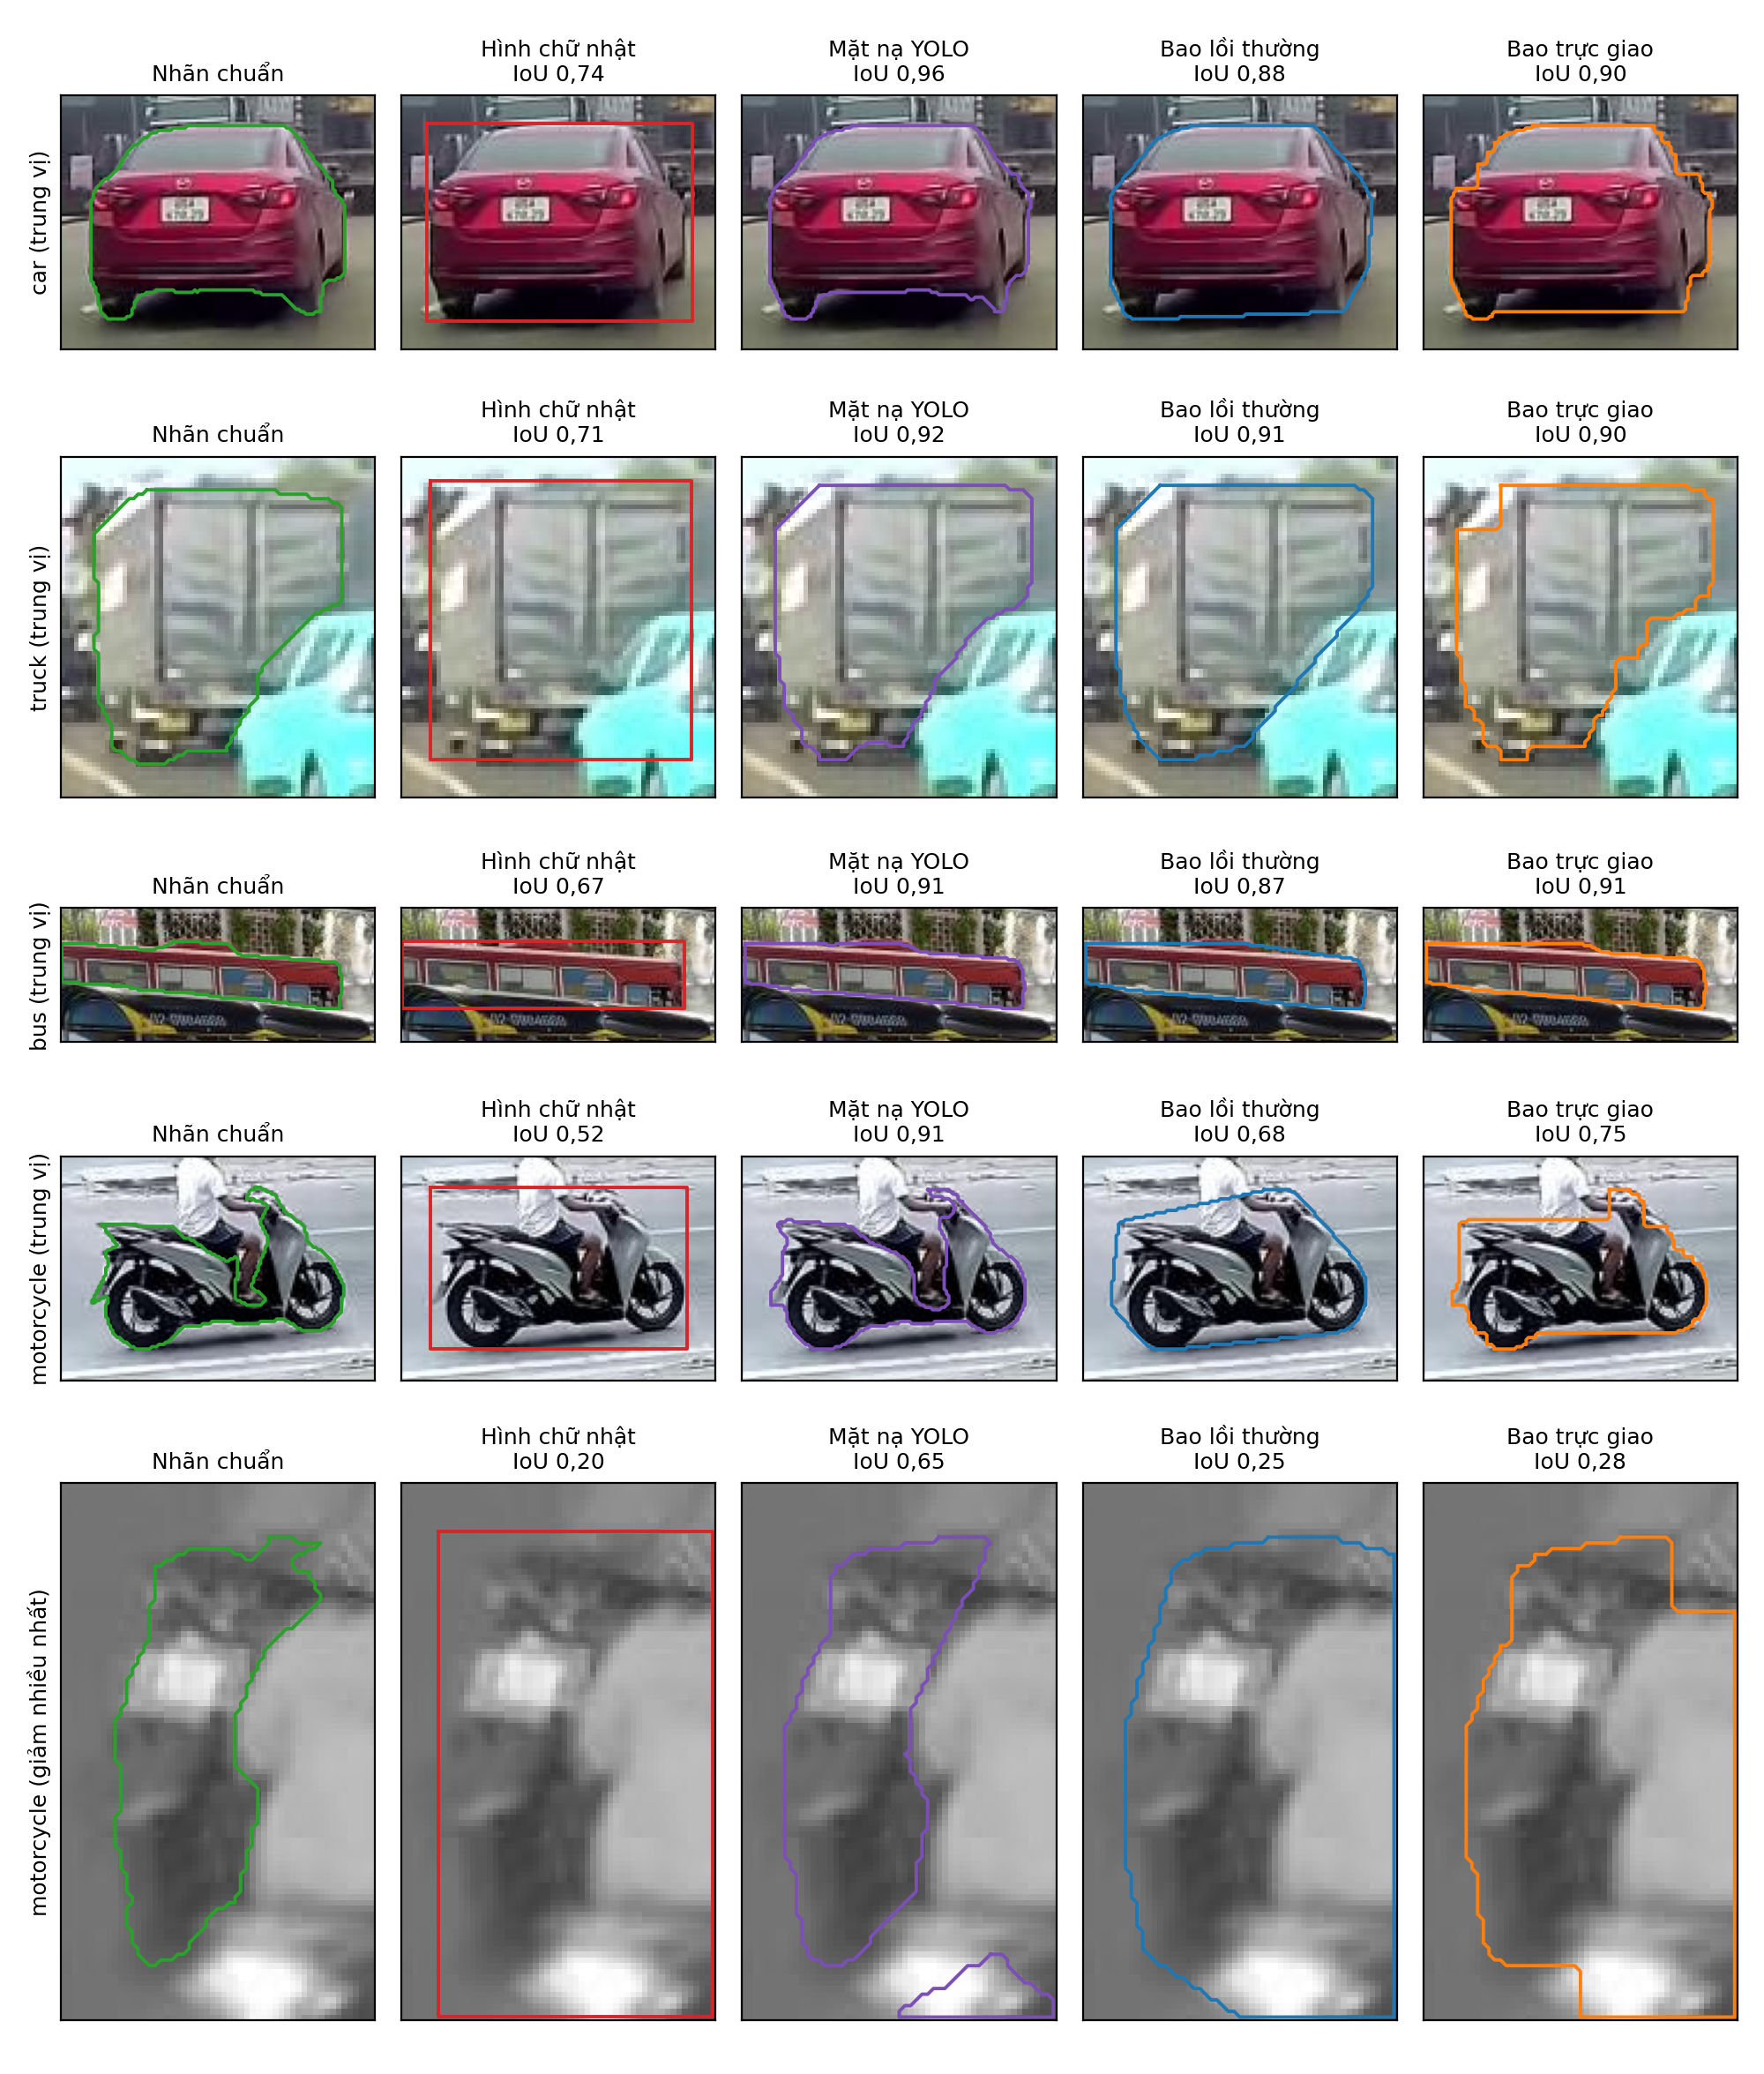
\includegraphics[width=\textwidth]{crop_compare.png}
\caption{Cùng một xe và cùng khung cắt, YOLO11-l trên bộ Việt Nam; IoU so với cùng nhãn. Chọn từ 219 cặp ghép đúng có nhãn từ 1\,600 điểm ảnh trở lên:
bốn hàng đầu là xe có IoU bao trực giao ở trung vị của từng lớp, hàng cuối là ca bao giảm IoU nhiều nhất so với mặt nạ. Đây là ví dụ minh hoạ, không đại diện cho xe nhỏ.}
\label{fig:crops}
\end{figure}

% =====================================================================
\section{Kết quả định tính}
\label{sec:qualitative}

Hình~\ref{fig:scenes} chọn ảnh theo F1 của mặt nạ YOLO trên bộ Việt Nam. Mỗi hàng gồm nhãn chuẩn (xanh dương), mặt nạ YOLO và bao trực giao.
Màu xanh lá là dự đoán đúng (TP), đỏ là dự đoán sai (FP), cam là nhãn bị bỏ sót.

\begin{figure}[H]
\centering
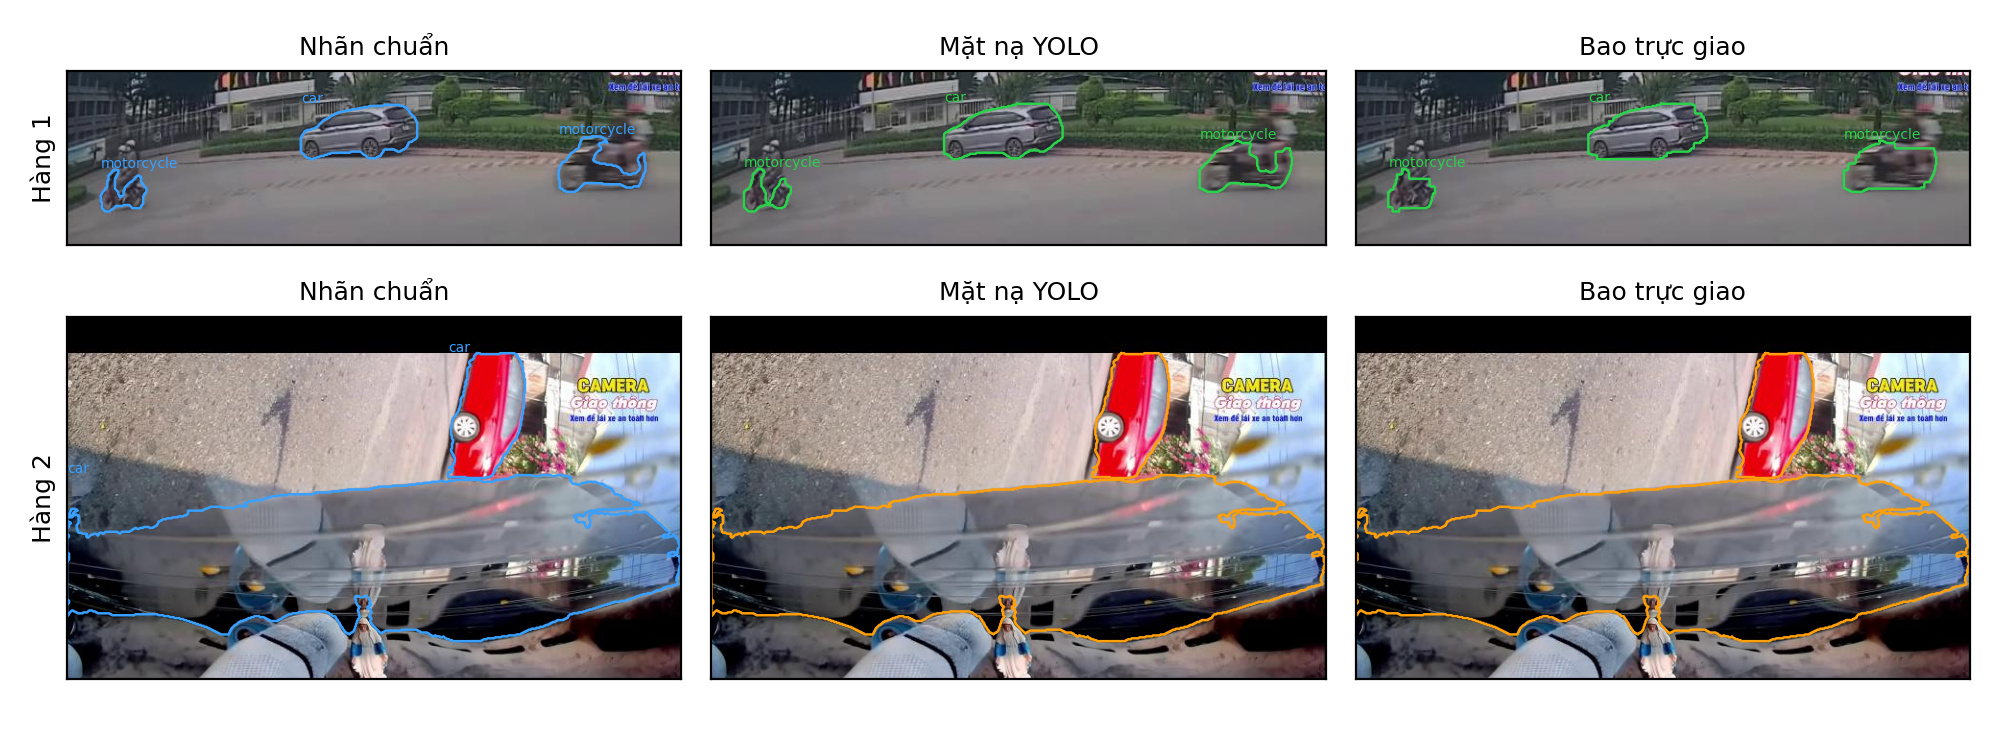
\includegraphics[width=\textwidth]{scene_compare.png}
\caption{YOLO11-l, bộ Việt Nam, độ tin cậy $\ge 0{,}20$. Hàng 1: ảnh dễ có F1 cao nhất. Hàng 2: ảnh khó có F1 thấp nhất, gồm một nhãn \texttt{car} đặt nhầm lên táp-lô
và một xe ở mép ảnh bị cắt, mô hình không phát hiện được.}
\label{fig:scenes}
\end{figure}

\paragraph{Minh hoạ trên video.}
Hệ thống dùng YOLO11-l kết hợp ByteTrack có sẵn trong Ultralytics để gắn ID, rồi dựng bao cho các xe có ID và mặt nạ. Hình~\ref{fig:video} được chọn ở khoảng giây thứ 5,2 của video ban đêm, sau khi xử lý một đoạn liên tiếp 36 khung hình bằng YOLO11-l và ByteTrack; bao được vẽ bằng bản Graham. Đây là minh hoạ chức năng, không phải phép đánh giá độ chính xác theo vết hay tốc độ toàn hệ thống; video không có nhãn ID chuẩn.

\begin{figure}[H]
\centering
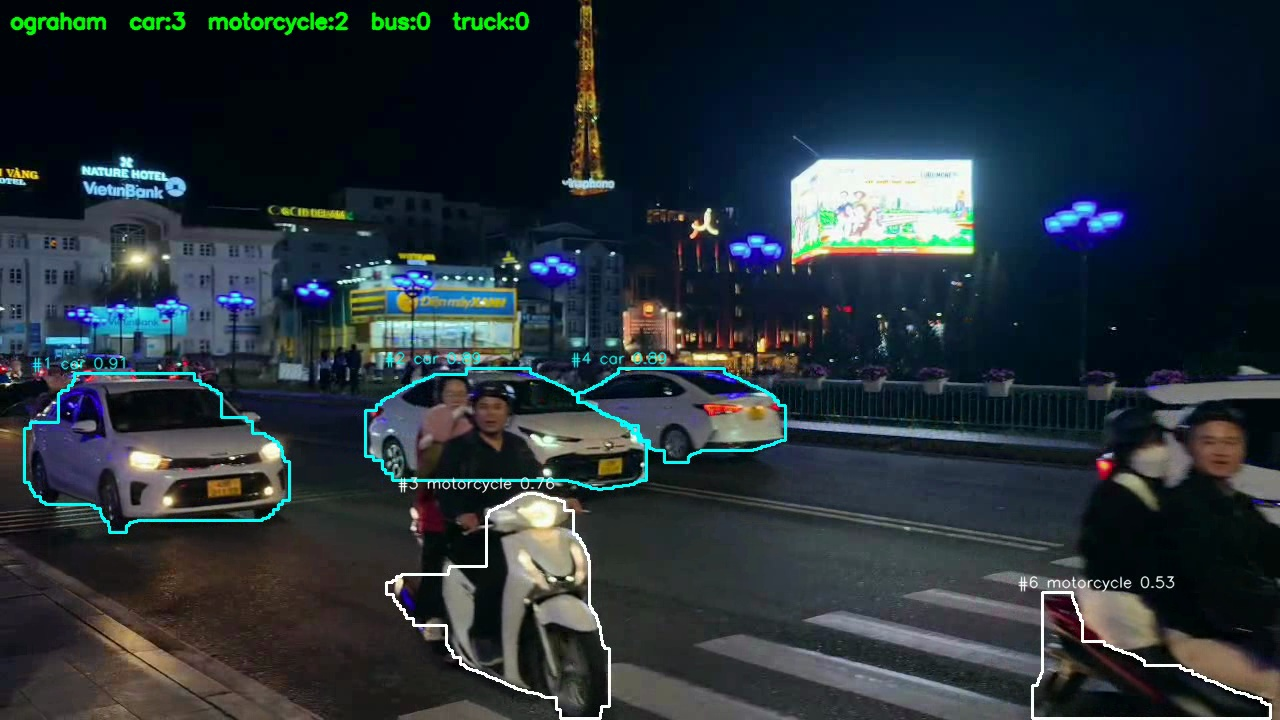
\includegraphics[width=\textwidth]{video_preview_night.jpg}
\caption{Đầu ra YOLO11-l kết hợp ByteTrack trên video giao thông ban đêm do nhóm cung cấp; bao được vẽ bằng bản Graham. Mỗi xe được hiển thị ID, lớp, độ tin cậy và vùng bao. Các số đếm ở góc trên là số đối tượng đang được hiển thị trong khung hình, không phải tổng số xe đi qua.}
\label{fig:video}
\end{figure}

% =====================================================================
\section{Thảo luận}
\label{sec:discussion}

\paragraph{Lựa chọn bản cài đặt.} Hai bản cài đặt cho cùng một bao trên dữ liệu thử, nên lựa chọn dựa trên tốc độ. Trong hai bản được khảo sát,
nhóm chọn O-Graham vì nhanh hơn trên đường biên xe và không chậm đi khi bao nhiều đỉnh. Đây là so sánh giữa hai bản cài đặt của nhóm,
không phải kết luận về O-Quickhull gốc: bài báo~\cite{nguyen2022quickhull} cho thấy O-Quickhull nhanh hơn O-Graham trên phần lớn dữ liệu họ thử.

\paragraph{Phạm vi sử dụng bao lồi trực giao.} Mặt nạ YOLO vẫn khớp nhãn tốt nhất ở mức điểm ảnh.
Bao lồi trực giao phù hợp khi cần một vùng \emph{liên thông, không lỗ}, có diện tích và chu vi tính trực tiếp, và sát nhãn hơn hình chữ nhật và bao lồi thường.
Các ứng dụng như ước lượng diện tích mặt đường bị chiếm hay kiểm tra va chạm vùng giữa các xe là hướng có thể dùng, nhưng chưa được đánh giá trong đồ án.

\paragraph{Giới hạn của đánh giá.}
\begin{itemize}
  \item Bộ 100 ảnh Việt Nam được chọn có chủ đích (70\% ảnh dễ), nhiều ảnh trích từ cùng một video nên có tương quan;
        kết quả không đại diện ngẫu nhiên cho giao thông Việt Nam.
  \item Nhóm đã thử fine-tune trên dữ liệu Việt Nam nhưng chưa ghi nhận cải thiện; các kết quả trong chương này sử dụng mô hình huấn luyện sẵn.
  \item Chưa khảo sát ảnh hưởng của kích thước đầu vào: ảnh $640\times640$ được phóng lên \texttt{imgsz=960} khi inference.
  \item Nhãn còn một số lỗi chưa sửa, được phát hiện khi xem trực quan: bộ Việt Nam có 7 xe van gán \texttt{car},
        khoảng 34 polygon nghi chỉ phủ một phần xe (22 ca là xe máy) và 4 nhãn đặt nhầm lên táp-lô hoặc gương xe. Polygon thiếu làm giảm recall xe máy:
        tính theo hộp, YOLO11-l đạt 61,8\% ở ngưỡng IoU 0,5 và 68,9\% ở ngưỡng 0,3.
\end{itemize}

\chapter{Kết luận và hướng phát triển}
\label{chap:conclusion}

\section{Kết quả đạt được}

Đồ án đã đưa bài toán tìm bao lồi trực giao liên thông vào ứng dụng phân đoạn phương tiện giao thông.

\paragraph{Về lý thuyết.} Đồ án trình bày khái niệm tập lồi trực giao, bao lồi trực giao và bao lồi trực giao liên thông,
cấu trúc bốn chuỗi bậc thang của bao và quan hệ bao hàm của bao với hình chữ nhật bao (Nhận xét~\ref{rem:inclusion}).
Đồ án tham khảo các nghiên cứu O-Quickhull \cite{nguyen2022quickhull} và O-Graham \cite{an2021ograham}, đồng thời trình bày hai bản cài đặt thực tế của nhóm:
bản O-Graham đạt $O(n\log n)$; bản QuickHull lấy cảm hứng từ O-Quickhull, nhanh khi bao ít đỉnh nhưng có trường hợp xấu $O(n^2\log n)$.

\paragraph{Về sản phẩm.} Đồ án xây dựng được chuỗi xử lý nhận dạng và dựng bao trên ảnh và video, kèm bộ kiểm thử tự động và bộ đánh giá có thể tái lập. Trên video, hệ thống dùng ByteTrack có sẵn trong Ultralytics để gắn ID trước khi dựng và hiển thị bao.

\paragraph{Về thực nghiệm.}
\begin{itemize}
  \item \textbf{Chọn mô hình.} So sánh sơ bộ cho thấy YOLO11-l cho mặt nạ tốt hơn YOLO11-n ở mọi chỉ số đã đo, rõ nhất ở recall xe máy (65,3\% so với 41,3\%), nên được chọn cho các thí nghiệm.
  \item \textbf{CH1.} Với mặt nạ chuẩn, bao lồi trực giao giữ IoU trung bình 94,8\%, cao hơn bao lồi thông thường (87,9\%) và hình chữ nhật
        (70,1\%).
  \item \textbf{CH2.} Hai bản cài đặt cho \emph{cùng một bao} trên mọi dữ liệu thử nghiệm, nên có chất lượng như nhau.
        Bản Graham nhanh hơn khoảng 1,4 lần theo thời gian trung vị trên đường biên xe thật và tới khoảng 40 lần ở trường hợp xấu
        với 10\,000 điểm. Nhóm chọn bản này cho chuỗi xử lý; kết quả không phải so sánh với O-Quickhull gốc.
  \item \textbf{CH3.} Với YOLO11-l, thay mặt nạ bằng bao làm mAP50--95 giảm từ 55,1\% xuống 47,6\% và mAP50 từ 74,6\% xuống 71,4\%,
        nhưng vẫn cao hơn hình chữ nhật (58,3\% mAP50). Đổi lại, bao là một vùng liền khối, không lỗ, trong khi khoảng một phần năm mặt nạ bị đứt mảnh.
        Số đỉnh của bao chỉ giảm ít so với đường biên đã rút gọn.
\end{itemize}

\section{Hạn chế}
\begin{itemize}
  \item Nhóm đã thử fine-tune trên dữ liệu Việt Nam nhưng kết quả chưa cải thiện. Lượng dữ liệu còn ít so với số lượng tham số của mô hình; xe máy vẫn bị bỏ sót nhiều.
  \item Bộ đánh giá còn nhỏ (100 ảnh) và được chọn có chủ đích.
  \item Bao lồi trực giao lấp thêm khoảng 9\% điểm ảnh so với mặt nạ YOLO, làm giảm mAP50--95.
  \item Chưa đánh giá tốc độ toàn chuỗi xử lý sau khi tích hợp ByteTrack.
  \item Thuật toán viết bằng Python thuần, chưa tối ưu.
\end{itemize}

\section{Hướng phát triển}
\begin{enumerate}
  \item \textbf{Fine-tune mô hình} YOLO11-seg trên dữ liệu giao thông Việt Nam (đặc biệt là xe máy), với tách tập
        huấn luyện/kiểm tra theo video để ảnh từ cùng một video không xuất hiện ở cả tập huấn luyện và tập kiểm tra.
  \item \textbf{Cài đặt hiệu năng cao}: viết lại phần dựng bao bằng C++/Numba, hoặc xử lý đồng thời bốn chuỗi bậc thang và các đối tượng khác nhau.
  \item \textbf{Ứng dụng đặc trưng hình học} của bao (diện tích, tỉ lệ lấp đầy) để phân loại lại car/truck
        hoặc ước lượng mức chiếm dụng mặt đường.
\end{enumerate}


\bibliographystyle{ieeetr}
\bibliography{refs}

\appendix
\chapter{Mã nguồn và hướng dẫn chạy}
\label{app:run}

Mã nguồn và hướng dẫn cài đặt, chạy chương trình được cung cấp tại GitHub:
\url{https://github.com/levienbang/yolo11}.

\chapter{Kết quả chi tiết}
\label{app:results}

\section{AP theo lớp của bao lồi trực giao}

\begin{table}[H]
\centering
\caption{mAP50 / mAP50--95 theo lớp (bao lồi trực giao, YOLO11-l)}
\begin{tabular}{lc}
\toprule
Lớp & mAP50 / mAP50--95 \\
\midrule
car        & 78,3 / 57,0 \\
truck      & 67,7 / 49,7 \\
bus        & 77,9 / 56,1 \\
motorcycle & 61,7 / 27,8 \\
\bottomrule
\end{tabular}
\end{table}

\section{Ảnh hưởng của ngưỡng độ tin cậy}

\begin{table}[H]
\centering
\caption{Precision / Recall của mặt nạ YOLO11-l theo ngưỡng độ tin cậy}
\begin{tabular}{rc}
\toprule
Ngưỡng & Precision / Recall \\
\midrule
0,05 & 45,0\% / 79,6\% \\
0,10 & 59,1\% / 75,6\% \\
0,20 & 74,9\% / 71,7\% \\
0,30 & 82,6\% / 66,9\% \\
0,50 & 89,2\% / 55,2\% \\
0,70 & 94,1\% / 38,5\% \\
\bottomrule
\end{tabular}
\end{table}

Ngưỡng 0,20 được chọn làm điểm cân bằng giữa Precision và Recall.


\end{document}
